\documentclass[11pt]{article}

% ====================================================
% PACKAGES
% ====================================================
\usepackage[margin=1in, headheight=13.6pt]{geometry}
\usepackage[T1]{fontenc}
\usepackage{lmodern}
\usepackage{microtype}
\usepackage{setspace}
\usepackage{tcolorbox}
\tcbuselibrary{skins,breakable}
\usepackage{amsmath, amssymb, mathtools}
\usepackage{siunitx}

\usepackage{graphicx}
\usepackage{float}
\usepackage{subcaption}

\usepackage{enumitem}
\usepackage{booktabs}
\usepackage{longtable}
\usepackage{array}
\usepackage{multirow}
\usepackage{ragged2e}

\usepackage{xcolor}
\usepackage{hyperref}

\usepackage{fancyhdr}
\usepackage{lastpage}

\usepackage{listings}
\usepackage{indentfirst}
\usepackage[justification=centering]{caption}
\usepackage[toc,page]{appendix}

\pagestyle{fancy}
\fancyhf{}
\lhead{\Assignment\ |\ \course}
\rhead{\Name\ |\ \today}
\cfoot{Page \thepage\ of~\pageref{LastPage}}

\hypersetup{
    colorlinks,
    linkcolor={red!50!black},
    citecolor={blue!50!black},
    urlcolor={blue!80!black}
}

\newcommand{\Name}{Arael Anaya}
\newcommand{\Assignment}{4.1 Preliminary Design Report}
\newcommand{\course}{Space Robotics}

\newtcolorbox{gapbox}{
    breakable,
    colback=orange!8,
    colframe=orange!70!black,
    boxrule=0.8pt,
    arc=2pt,
    left=6pt, right=6pt, top=4pt, bottom=4pt,
    fonttitle=\bfseries,
    title={\textcolor{orange!70!black}{\Large\textbullet}\ GAP: Needs Author Input}
}

\newcommand{\reqid}[1]{\textbf{#1}}

\begin{document}

% ====================================================
% TITLE BLOCK
% ====================================================
\begin{center}
    {\LARGE\bfseries Preliminary Design Report}\\[4pt]
    {\Large A Multi-Agent Robotic System for Autonomous Ice-Shell}\\
    {\Large Characterization and Cryobot Site Selection on Europa}\\[10pt]
    {\large Arael Anaya}\\
    {\large Space Robotics: 4.1 Preliminary Design Report}\\
    {\large \today}
\end{center}

\newpage
\tableofcontents
\newpage

% ====================================================
% 1. EXECUTIVE SUMMARY
% ====================================================
\section{Executive Summary}

This mission deploys a coordinated multi-agent robotic system to Europa, Jupiter's icy moon, to
autonomously characterize ice-shell thickness along a surface traverse and identify an optimal
cryobot insertion site, operating without real-time Earth support~\cite{owlDecadal}. The system
consists of a surface rover carrying a ground-penetrating radar sounder, supported by two
orbital relay agents that provide terrain reconnaissance, communications relay, and cooperative
localization~\cite{nasaSBIR}. This mission directly addresses three converging research gaps:
autonomous operations in GPS-denied, high-radiation environments; multi-agent coordination and
interoperability for cooperative task planning~\cite{stmdShortfall}; and fully autonomous
approach and proximity operations without Earth-based navigational support~\cite{nasaSBIR}.

Europa was chosen as the destination because it holds strong indicators of conditions favorable
to life and contains the chemical building blocks necessary to support it~\cite{owlDecadal}. Its
subsurface ocean makes it one of the most promising locations in the Solar System for
astrobiology, but the 44-minute one-way light delay to Jupiter, Jupiter's intense radiation
environment, and a $90$~K cryogenic surface make it one of the most demanding environments to
operate a robot in. Every decision from landing onward must be made onboard; there is no
real-time human-in-the-loop safety net.

The rover is a four-wheel, differential-drive vehicle riding on a single-pivot rocker, sized
against a $147.25$~kg contingency mass cap, and powered by a Radioisotope Thermoelectric
Generator (RTG) rather than solar arrays, since solar irradiance at Europa's distance from the
Sun collapses to roughly $50\ \mathrm{W/m^2}$. Its primary payload is a REASON-heritage
dual-frequency, ice-penetrating radar sounder, the same instrument family currently flying
aboard NASA's Europa Clipper spacecraft~\cite{reason}. Where Clipper collects wide-swath,
low-resolution orbital snapshots of the ice shell, this mission's rover drives a continuous
surface traverse, building a spatially registered subsurface profile at $100$~m resolution or
better and autonomously flagging the thinnest viable ice for a future cryobot deployment.

Two orbital agents support the rover from a $200$~km circular Europa orbit, providing terrain
mapping ahead of the traverse, a UHF proximity relay for the rover's science and command
traffic, and an independent ranging source the rover can use to recover its position after a
localization fault. Communication with Earth exists only as a low-rate contingency beacon; a
direct link at Europa's distance closes at roughly $7$ bits per second, which is why the relay
architecture is not optional but foundational to the mission design.

Across a 30-sol surface mission, the system is expected to produce a continuous, georeferenced
subsurface ice-thickness profile along the traverse track, a validated candidate cryobot
insertion site (ice thickness under $5$~km, surface slope under $20^\circ$, terrain roughness
under $0.7$), and a full science and engineering telemetry archive suitable for both real-time
onboard decision-making and post-mission analysis by Earth-based planetary scientists. The
requirements, environmental analysis, concept of operations, payload rationale, data strategy,
and subsystem designs that support this objective are detailed in the sections that follow.

% ====================================================
% 2. RESEARCH CONTEXT AND GAP FRAMING
% ====================================================
\section{Research Context and Gap Framing}

Three converging research gaps motivate this mission, drawn from the OWL Planetary Decadal
Survey, a NASA STMD technology shortfall, and a NASA SBIR/STTR solicitation topic.

\subsection{OWL Decadal Survey: Ocean Worlds Exploration \& Sampling}

\textbf{Topic:} Ocean Worlds Exploration \& Sampling~\cite[pp.~36--39]{owlDecadal}

\textbf{Interest:} Ocean worlds like Europa represent the most compelling environments
for studying life beyond Earth, and the most difficult for autonomous systems. What draws me to
this topic is the engineering challenge that arises from the question: how do you keep a robot
operational, navigating, and decision-making in a GPS-denied, high-radiation, cryogenic
environment with no possibility of real-time human intervention? The decadal survey speaks to
the real physical needs here: Jupiter's Galilean moons reveal ``the fundamental importance of
gravitational tides in generating internal heat,'' with those tides actively ``melting ice on
Europa and Ganymede''~\cite[p.~37]{owlDecadal}. That subsurface ocean exists because of a
process we cannot turn off, and any robotic system sent to study it must be designed around that
reality.

\textbf{Connection to Space Exploration:} Accessing a subsurface ocean requires
penetrating kilometers of ice, a process that may yield in-situ resources (liquid water,
chemical energy gradients) critical to sustaining any long-duration mission. Understanding the
composition of that ocean directly informs the feasibility of using local materials to support
future human or robotic infrastructure in the outer solar system.

\textbf{Relationship to Robotics:} Reaching and operating in a subsurface ocean demands
a full robotic stack operating without outside reference: specialized robots for ice
penetration, underwater vehicles for ocean navigation, and autonomous sampling systems capable of
detecting and responding to scientifically interesting features. Every subsystem (perception,
localization, path planning, controls) must function independently.

\subsection{NASA STMD Shortfall: Multi-Agent Robotic Coordination}

\textbf{Topic:} Multi-Agent Robotic Coordination and Interoperability for Cooperative
Task Planning and Performance~\cite{stmdShortfall}

\textbf{Interest:} Swarm robotics is the next step in advancing the capabilities of
robots to complete high-level missions. NASA's own shortfall rankings confirm how urgent this is:
multi-agent coordination received an integrated score of $4.7856$ and ranked $139$th among all
civil space technology gaps~\cite{stmdShortfall}, placing it right in the near-term priority tier
for Autonomous Systems and Robotics. I am most interested in the version of it where each robot
in the swarm is genuinely capable on its own, not a simple unit that only functions within the
group, but a system of robots with unique capabilities that all come together to complete a
high-level task.

\textbf{Connection to Space Exploration:} Cooperative exploration and mapping by a
distributed robotic fleet dramatically increases the spatial coverage and fault tolerance of
resource missions. A swarm can survey a large asteroid surface, map subsurface ice deposits via
distributed sensing, or maintain constant monitoring of a volatile-rich region far more
efficiently than any single agent, with adversarial identification algorithms when individual
units fail.

\textbf{Relationship to Robotics:} This topic is a direct application of the consensus
and coordination algorithms I have studied for the last year. Deploying them in space introduces
new constraints (limited bandwidth, high latency, radiation-induced faults, and no GPS) that
stress-test the theoretical properties I've studied (convergence, resilience, scalability).

\subsection{NASA SBIR/STTR Topic: Flight Dynamics and Navigation Technologies}

\textbf{Topic:} Flight Dynamics and Navigation Technologies~\cite{nasaSBIR} (Topic
COMNAV.1.S26B)

\textbf{Interest:} Communication delays and blackouts are not random edge cases in
deep-space missions; they are the default operating condition. The SBIR solicitation states the
gap directly: ``NASA currently has limited navigational and guidance technologies that permit
fully autonomous approach, proximity operations, distributed spacecraft operations, and landing
without support from Earth-based resources''~\cite{nasaSBIR}. This shortfall interests me because
it forces onboard autonomy to be the primary decision-making layer, eliminating the safety net of
human-in-the-loop oversight.

\textbf{Connection to Space Exploration:} Remote resource operations (prospecting,
extraction, processing) cannot depend on continuous communication to Earth. Whether managing an
ISRU plant on the lunar surface or conducting a sampling traverse on an asteroid, the system must
detect anomalies, replan, and execute without waiting for human feedback.

\textbf{Relationship to Robotics:} My research in consensus algorithms and resilient
multi-agent coordination already deals with how distributed systems reach agreement under
adversarial conditions. Extending this to communication-constrained space contexts is a natural
progression: the same algorithms that allow a swarm of Crazyflies to maintain stability during
packet loss should also apply to a team of planetary rovers operating through a communication
outage.

% ====================================================
% 3. MISSION DEFINITION AND ENVIRONMENT
% ====================================================
\section{Mission Definition and Environment}

\subsection{Mission Objective \& Destination}

\textbf{Selected Research Gap:} While most robotic space missions have focused on a
single agent carrying all the capabilities needed to complete the mission objectives, the future
of advanced planetary exploration lies in multi-agent systems that are able to share
responsibility and support each other. In order to fully understand a body as complex as Europa,
it is necessary to divide surveying tasks across the main exploration rover and the orbital
agents needed to scout terrain ahead of it. This mission directly addresses three converging
research gaps: autonomous operations in GPS-denied, high-radiation environments~\cite{owlDecadal};
multi-agent coordination and interoperability for cooperative task planning~\cite{stmdShortfall};
and fully autonomous approach and proximity operations without Earth-based navigational
support~\cite{nasaSBIR}.

\textbf{Mission Statement:} The multi-agent Europa surface system shall autonomously
characterize the ice shell and identify a cryobot insertion site, operating without real-time
Earth support.

\textbf{Success Criteria (summary):} Full traverse track covered at $\leq 100$~m
along-track spacing, ice-thickness accuracy within $\pm 10\%$ against calibration targets, and
at least one candidate insertion site flagged by the onboard algorithm (ice thickness $<5$~km,
surface slope $<20^\circ$, terrain roughness $<0.7$). Section~3.3 develops the full mission- and
operations-level requirements that this criterion is built from.

\textbf{Destination Justification:} My mission takes place on Europa, Jupiter's icy
moon. I chose this destination due to the abundance of knowledge there is to gain from an
in-depth exploration of the system. Europa holds strong indicators of conditions favorable to
life and contains all the chemical building blocks necessary to support it~\cite{owlDecadal}.
The layers of ice introduce in-situ resources that might benefit further exploration of the moon
as long-term infrastructure is developed, as well as imposing significant rover design
constraints. Any surface vehicle must feature traction-optimized wheels capable of accurately
traversing the fractured, chaotic terrain.

Europa is also incredibly challenging. The 44-minute one-way light delay means every decision
from landing onward must be fully autonomous~\cite{nasaSBIR}. Due to the intense radiation
environment driven by Jupiter's magnetosphere, the rover relies on orbiting satellite robots to
scan the terrain and share terrain maps prior to surface traversal. Such a system has to be
highly robust to faulted or adversarial agents, as incorrect or incomplete maps shared across
the swarm are likely to produce dangerous navigation decisions. This location is essential to the
mission because it provides an incredibly challenging environment that necessitates smart,
advanced robot design and algorithm development, the perfect stage to push robotic
capabilities to their limits.

\subsection{Environmental \& Operational Challenges}

Europa's environment is hostile in ways that shape every design decision in this mission.
Jupiter's magnetosphere floods the moon's surface with high-energy charged particles, exposing
electronics to radiation doses far greater than what commercial components can tolerate. This
motivates a requirement for radiation-hardened electronics and a shielded vault setup for the
rover's core computing hardware, similar to the approach taken on the Galileo
spacecraft~\cite{owlDecadal}. Redundancy at the agent level is an equally important mitigation:
if one surface relay node builds up enough single-event upsets to go silent, the remaining agents
must autonomously reconfigure the network to maintain coverage.

Surface temperatures on Europa are around $90$~K, which introduces thermal management challenges
for both batteries and actuators. Power storage capacity drops significantly at cryogenic
temperatures, meaning the rover must actively manage its thermal systems to keep cells within an
operational range rather than simply relying on passive insulation. Solar power is not viable at
Europa's distance from the Sun (irradiance collapses to roughly $50\ \mathrm{W/m^2}$), so the
system instead relies on an RTG.

The complete absence of GPS and the communication blackout imposed by the 44-minute light delay
mean the swarm cannot depend on any external reference for localization or replanning. Each agent
must maintain its own state estimate using onboard sensors and inter-agent ranging, and the swarm
must reach consensus on shared map data using algorithms that are resilient to packet loss and
radiation-induced faults~\cite{stmdShortfall,nasaSBIR}. There is no human in the loop to catch a
bad map before the rover commits to a traverse. Table~\ref{tab:env-drivers} summarizes how each
environmental driver maps onto a subsystem-level design response; the full derivation appears in
the subsystem sections of Section~7.

\begin{table}[H]
\centering
\small
\begin{tabular}{p{4cm}p{4.5cm}p{5.5cm}}
\toprule
\textbf{Environmental Driver} & \textbf{Operational Consequence} & \textbf{Design Response} \\
\midrule
Jupiter magnetosphere radiation ($\geq 100$~krad) & Electronics degradation, single-event upsets & Radiation vault (Ti-6Al-4V + Pb/poly liner), agent-level redundancy \\
44-min one-way light delay & No real-time human command & Full onboard autonomy, consensus-based multi-agent decisions \\
No GPS, no magnetic field & No absolute position/heading reference & Visual odometry + IMU + fine sun sensors + inter-agent ranging \\
$90$~K cryogenic surface & Battery capacity loss, actuator lubricant stiffening, brittle materials & MLI + RTG waste-heat routing + survival heaters, pre-motion warm-up \\
$\sim 50\ \mathrm{W/m^2}$ solar irradiance & Solar arrays not viable & RTG primary power source \\
Fractured, chaotic ice terrain & Traction/mobility risk, hazard density & Cleated wheels, onboard hazard rejection, low-speed arc-based traversal \\
\bottomrule
\end{tabular}
\caption{Environmental drivers and their design responses.}
\label{tab:env-drivers}
\end{table}

\subsection{Mission Success Criteria}

Requirements are drawn from the master requirements spreadsheet (Appendix~B contains the full
set, REQ.01.01 through REQ.12.04). Table~\ref{tab:mission-level-reqs} presents three
mission-level requirements and Table~\ref{tab:ops-level-reqs} presents three operations-level
requirements, each with its justification, verification approach, and associated risk.

\begin{table}[H]
\centering
\small
\begin{tabular}{p{1.5cm}p{5.3cm}p{4cm}p{3.2cm}}
\toprule
\textbf{ID} & \textbf{Statement} & \textbf{Justification} & \textbf{Verification / Risk} \\
\midrule
REQ.01.01 &
The multi-agent Europa system shall operate fully autonomously for the entire surface mission
duration without requiring real-time command uplinks from Earth. &
The 44-minute one-way light delay makes real-time commanding physically impossible; all
decisions must be onboard. &
72-hr hardware-in-the-loop mission sequence with a simulated blackout, zero unresolved Earth
dependencies. Risk-01: single-point autonomy failure with no fallback human override. \\
\addlinespace
REQ.01.02 &
The system shall survive and maintain operational status after exposure to a total ionizing dose
of no less than $100$~krad over the nominal mission lifetime. &
Jupiter's magnetosphere delivers doses far exceeding near-Earth missions; Europa Clipper's
radiation vault targets $\sim 100$~krad as its design threshold. &
Co-60 gamma irradiation of radiation-sensitive components to $110$~krad ($10\%$ margin) with
functional monitoring throughout. RISK-02: accumulated SEUs degrade consensus convergence before
mission completion. \\
\addlinespace
REQ.01.03 &
The system shall maintain a minimum inter-agent network connectivity of two active relay nodes
at all times during surface operations to ensure consensus is achievable. &
Consensus algorithms require a minimum connected graph; two relays plus the rover guarantee a
3-node connected topology, the minimum viable configuration. &
Network fault simulation with progressive relay failures; reconfiguration must trigger before
dropping below 2 active nodes. RISK-03: simultaneous radiation-induced failure of multiple relay
nodes isolating the rover. \\
\bottomrule
\end{tabular}
\caption{Mission-level requirements.}
\label{tab:mission-level-reqs}
\end{table}

\begin{table}[H]
\centering
\small
\begin{tabular}{p{1.5cm}p{5.3cm}p{4cm}p{3.2cm}}
\toprule
\textbf{ID} & \textbf{Statement} & \textbf{Justification} & \textbf{Verification / Risk} \\
\midrule
REQ.02.01 &
The surface robot shall maintain a localization accuracy of no worse than $\pm 0.5$~m relative
to its last known position during traverse segments up to $50$~m in the absence of GPS. &
Cryobot insertion site selection requires meter-level positioning to match the radar-identified
thin-ice candidate; consistent with visual odometry performance on Mars rovers. &
Analog-terrain field test, 50~m commanded segments, onboard estimate vs.\ ground truth across 20
runs. RISK-04: ice surface texture homogeneity reducing visual odometry feature tracking. \\
\addlinespace
REQ.03.01 &
The ground-penetrating radar sounder shall resolve ice shell thickness to within $\pm 10\%$
accuracy for ice layers between $1$~km and $30$~km depth, producing a subsurface map at a
minimum spatial resolution of $100$~m along the traverse track. &
Identifying the optimal cryobot insertion site requires knowing where the ice shell is
thinnest; consistent with Europa Clipper REASON design parameters. &
Laboratory radar range measurements against known-thickness ice-analog targets across the full
depth range. RISK-05: ice-shell heterogeneity or brine inclusions creating radar clutter. \\
\addlinespace
REQ.04.01 &
The inter-agent mesh network shall achieve consensus on a shared terrain map update within no
more than $10$~minutes under a degraded network condition of up to $30\%$ packet loss on any
single inter-agent link. &
Traverse planning depends on a current, consensus-validated terrain map; a 10-minute bound keeps
planning delay acceptable, and $30\%$ loss is a plausible radiation-induced degradation
scenario. &
Software-in-the-loop consensus simulation, $30\%$ packet loss injected on every link across 100
test runs. RISK-06: radiation-induced burst errors exceeding $30\%$ loss on multiple links
simultaneously, stalling consensus. \\
\bottomrule
\end{tabular}
\caption{Operations-level requirements.}
\label{tab:ops-level-reqs}
\end{table}

\textbf{Not applicable.} The master spreadsheet marks every requirement's \emph{Status} field as
``Unaccomplished.'' This is expected rather than an open item: this is a paper design exercise
with no physical rover or relay hardware built, so no requirement can be verified by analysis,
test, or demonstration in the sense the V\&V columns call for, and the Status field is left
accurate as-is.

% ====================================================
% 4. CONCEPT OF OPERATIONS (CONOPS)
% ====================================================
\section{Concept of Operations (ConOps)}

\subsection{Overview Narrative}

The multi-agent system deployed to Europa's surface autonomously characterizes ice shell
thickness and identifies an optimal cryobot insertion site without real-time Earth support. The
destination is Europa, chosen because its subsurface ocean makes it one of the most promising
locations in the Solar System for astrobiology and future exploration. The mission deploys a
surface rover equipped with a ground-penetrating radar sounder, supported by two orbital
reconnaissance agents that provide terrain mapping, communications relay, and cooperative
localization. By leveraging radar sounding techniques analogous to the Europa Clipper REASON
instrument, the system generates detailed subsurface ice maps to support future cryobot missions.

The mission consists of six main phases: Launch and Commissioning, Cruise and Approach, Europa
Orbit Insertion and Reconnaissance, Landing, Surface Checkout and Site Characterization, Surface
Survey and Ice Characterization, and End-of-Mission Operations. Launch and cruise prepare the
system for arrival at Europa. Upon arrival, the orbital agents conduct reconnaissance and
identify a suitable landing region. Landing is followed by rover deployment, system checkout, and
sensor calibration. Main surface operations focus on autonomous rover traversal while collecting
radar measurements of the ice shell and building a subsurface map; the orbital agents
continuously update terrain maps and relay communications. The final phase includes science data
downlink, candidate cryobot site selection, optional extended operations, and safe system
passivation.

The rover operates autonomously during critical events such as landing, navigation, radar
sounding, and site-selection activities. The two orbital agents provide terrain reconnaissance,
communications relay, cooperative localization support, and validation of shared mapping data.
Ground teams remain in the loop during cruise, strategic mission planning, and anomaly
resolution, but all tactical decisions must be performed onboard due to the approximately
$43$--$44$ minute one-way communication delay between Earth and Jupiter. Radiation exposure,
cryogenic temperatures, communication delays, and limited bandwidth are the key operational
constraints that shape every phase below.

\subsection{Operational Timeline}

Table~\ref{tab:conops-timeline} presents the mission-phase-level ConOps timeline (mission phases,
operation modes, and key events), and Figure~\ref{fig:conops-flow} presents the corresponding
operational flow graphic. A finer-grained, minute-by-minute breakdown for the first three sols of
surface operations plus the steady-state daily cycle and end-of-mission sequence is maintained in
the source spreadsheet (\textit{2.4 ConOps Detailed Timeline}); it is summarized in
Table~\ref{tab:conops-daily-cycle} rather than reproduced row-by-row here for length.

\begin{table}[H]
\centering
\footnotesize
\begin{tabular}{p{1.6cm}p{2.6cm}p{3.3cm}p{1.4cm}p{2cm}p{2.5cm}}
\toprule
\textbf{Time} & \textbf{Mode} & \textbf{Objective / Milestone} & \textbf{Op. Mode} &
\textbf{Risk} & \textbf{Duration} \\
\midrule
Launch day, 0--1 & Launch \& Commissioning & Spacecraft separation, initial health checks &
Scripted/Auto & High & 1 day \\
Cruise, yrs 0--6 & Cruise \& Approach & Maintain health, trajectory correction maneuvers &
Semi-Auto & Medium & $\sim$6 years \\
Europa arrival & Orbit Insertion \& Reconnaissance & Deploy orbital agents, identify landing
region & Autonomous & High & 30 days \\
Surface day 0--5 & Landing, Checkout \& Site Characterization & Deploy rover, verify health,
calibrate payload & Autonomous & High & 5 days \\
Surface day 5--35 & Surface Survey \& Ice Characterization & Map subsurface ice, identify
candidate cryobot sites & Autonomous & Medium & 30 days \\
Surface day 35--50 & Data Transmission \& End of Mission & Downlink archive, select final site,
passivate & Semi-Auto & Low & 15 days \\
\bottomrule
\end{tabular}
\caption{Mission-phase-level Concept of Operations timeline.}
\label{tab:conops-timeline}
\end{table}

\begin{figure}[H]
    \centering
    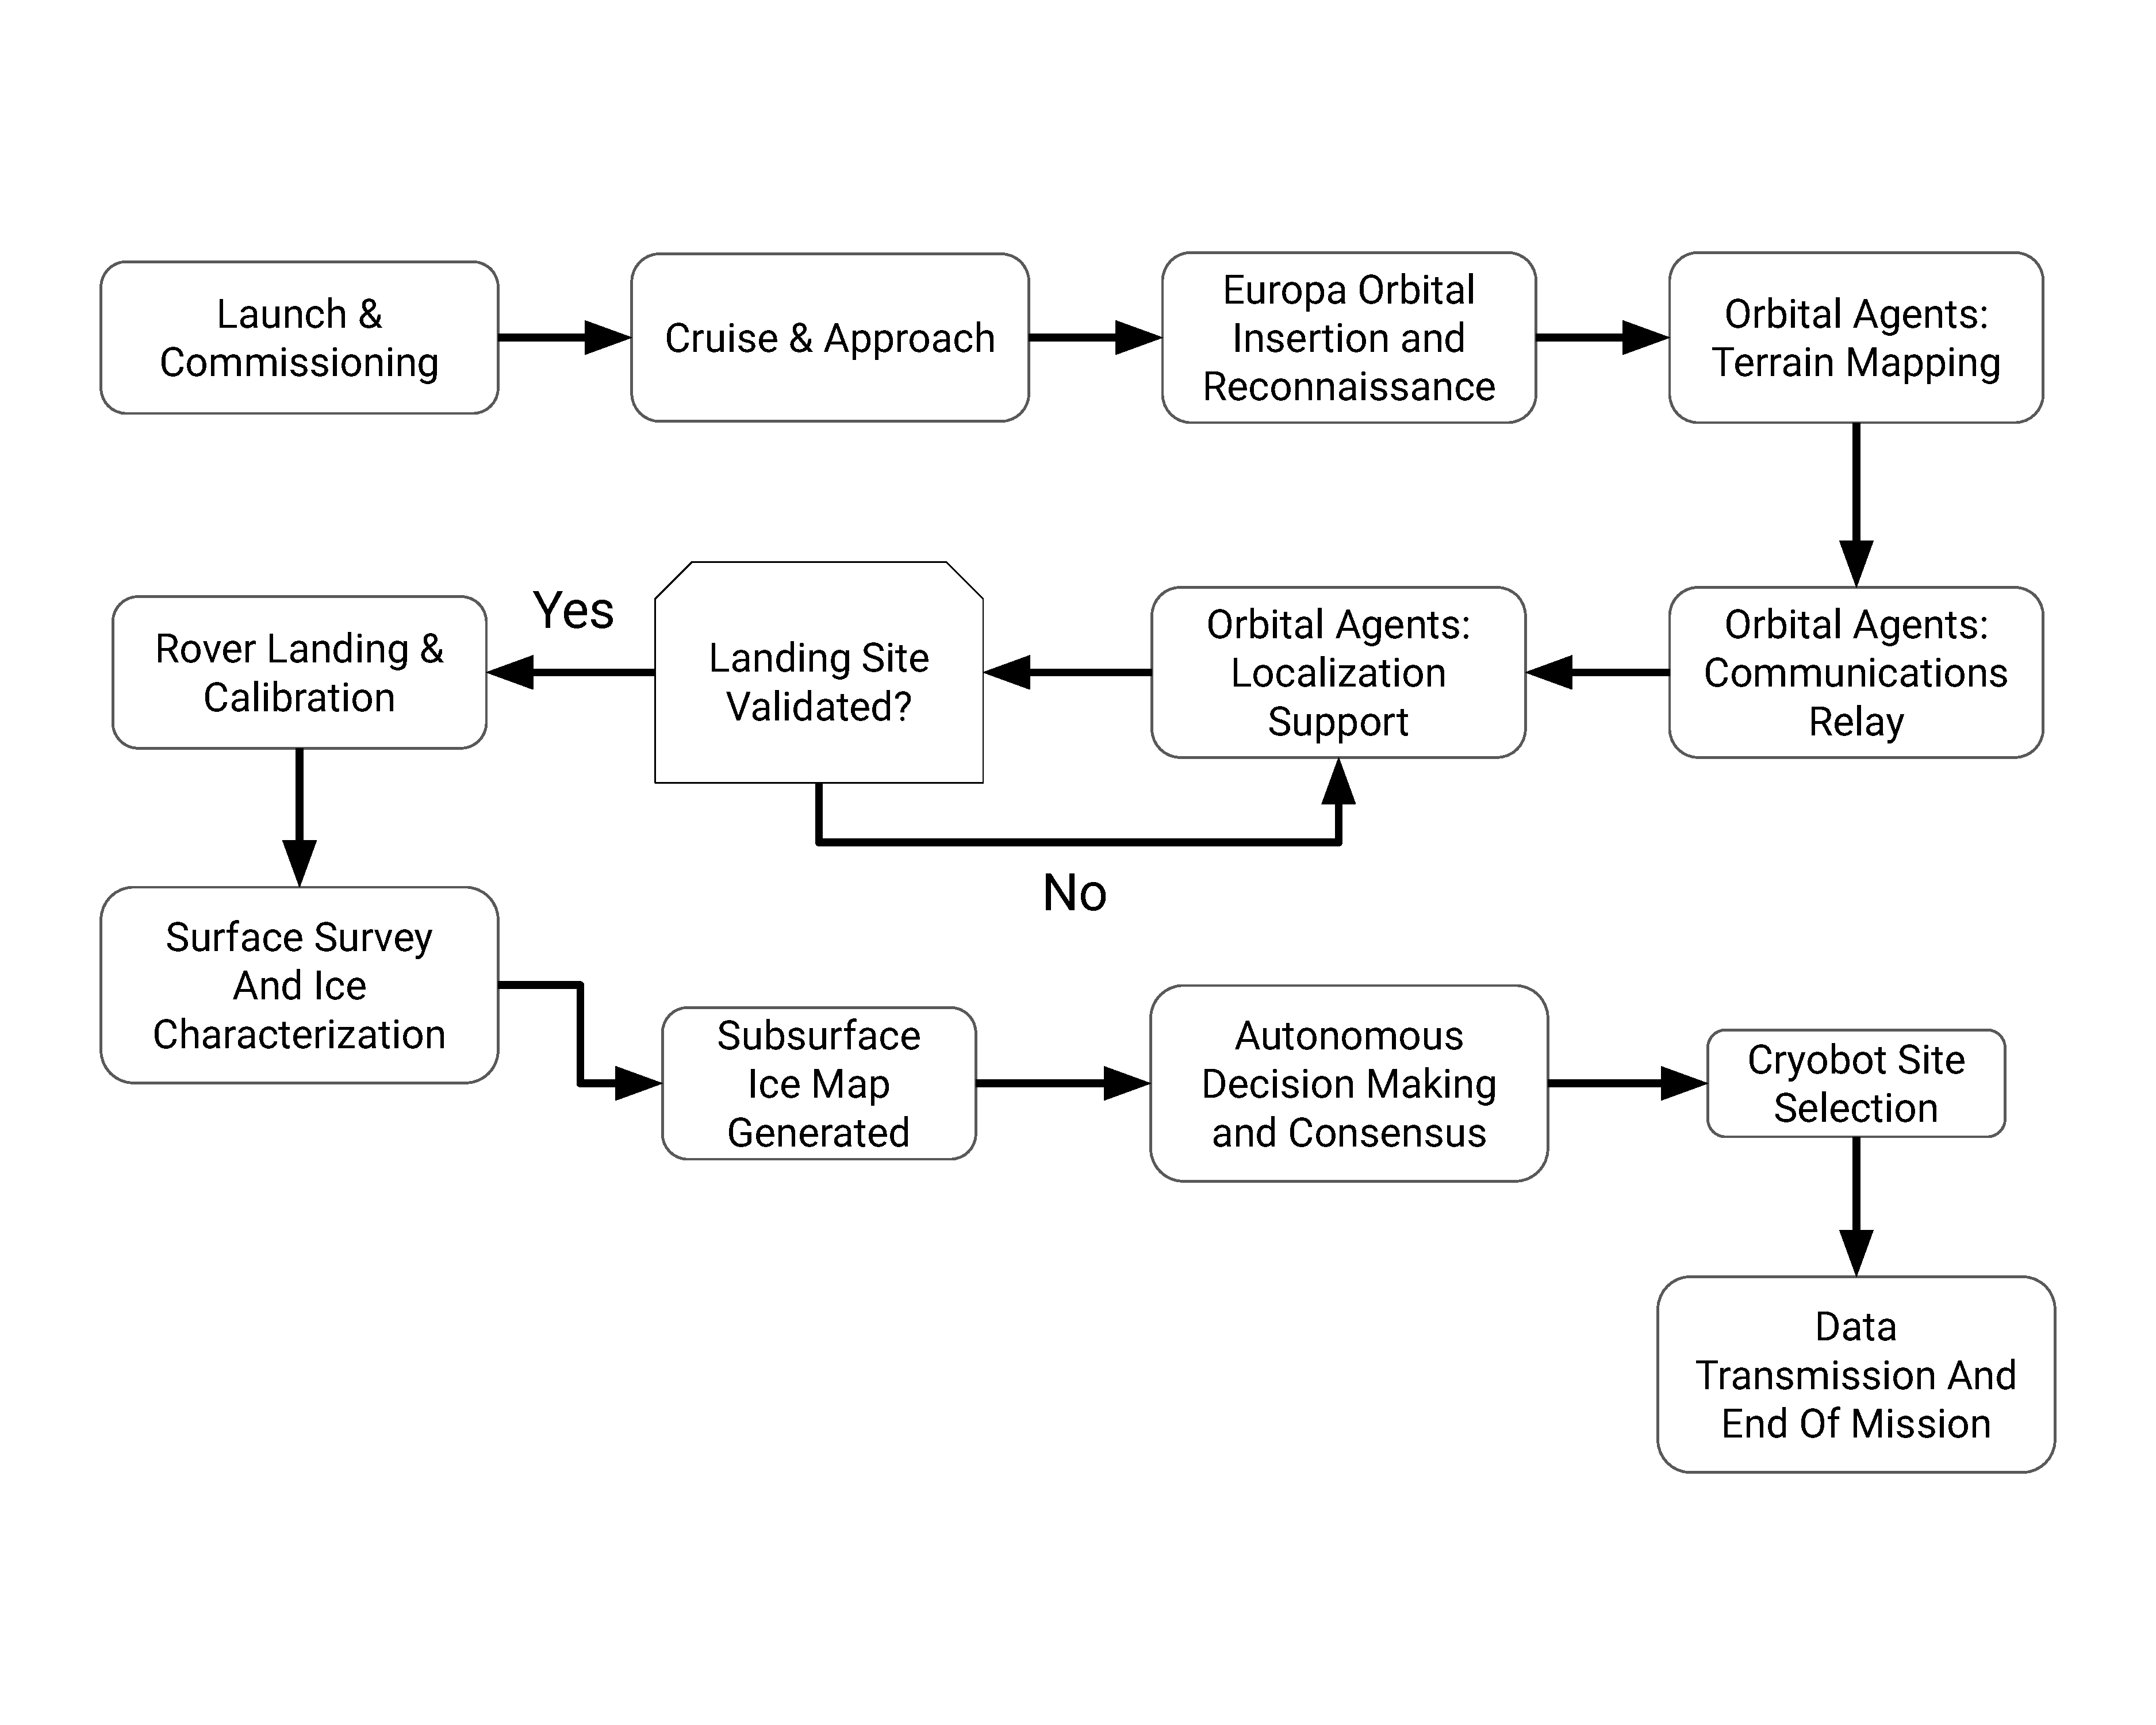
\includegraphics[width=0.85\textwidth]{figures/conops_flow.pdf}
    \caption{Operational flow across the six mission phases, including the landing-site
    validation decision point and the autonomous consensus loop that drives cryobot site
    selection.}
    \label{fig:conops-flow}
\end{figure}

\begin{table}[H]
\centering
\footnotesize
\begin{tabular}{p{2cm}p{2.2cm}p{9cm}}
\toprule
\textbf{Sol(s)} & \textbf{Phase} & \textbf{Key Events} \\
\midrule
0 & Initialization & Descent/landing ($0$--30 min); commissioning and health checks; orbital comms
verification; localization initialization; radar payload init, calibration, and validation;
initial site characterization; night low-power thermal management. \\
1--2 & Activation & Daily cycle established: autonomous traverse planning, orbital terrain
mapping update, surface survey blocks, localization verification, radar data collection,
communications relay pass, subsurface ice map generation. \\
3--25 & Steady-state operations & Repeating daily cycle: traverse planning $\to$ survey
operations $\to$ radar data collection $\to$ communications relay pass $\to$ subsurface ice map
update $\to$ night low-power thermal management. \\
26--28 & Site selection & Candidate site ranking and autonomous consensus validation (repeated
over two sols), final site assessment, cryobot site selection. \\
29 & Archive \& validation & Final science archive generation, final terrain map validation. \\
30 & End of mission & Final data dump, rover/payload safing, communications shutdown,
passivation and final health beacon. \\
\bottomrule
\end{tabular}
\caption{Summary of the minute-by-minute surface operations timeline (source: 2.4 ConOps
Detailed Timeline spreadsheet).}
\label{tab:conops-daily-cycle}
\end{table}

\subsection{Flight Software State Diagram}

Figure~\ref{fig:conops-state-flow} presents the flight-software state flow (source: \textit{2.5
ConOps State Flow Diagram}), covering all six mission phases from Launch and Cruise through End
of Mission. Each rover-state block (purple) is bounded by an orbital-agent or ground-command
dependency where one exists (e.g., \textsc{Orbital Terrain Mapping \& Localization} gates
\textsc{Landing Validated?} before Phase 3 begins), and every conditional branch resolves to a
named exit rather than an implicit fall-through: a failed landing confirmation routes to
\textsc{Safe Mode}, an out-of-tolerance slope check during Phase 4 traverse planning routes to
\textsc{Halt Traversal}, and a sub-10-minute consensus failure on the relay pass retries rather
than proceeding on stale data (REQ.04.01). The Phase 4 steady-state block (Traverse Planning
$\to$ Survey/Sounding $\to$ Slope Check $\to$ Relay Pass $\to$ Consensus Check $\to$ Map Update
$\to$ Night Low-Power) loops for sols 1--25 before handing off to Phase 5 site selection, matching
the daily cycle in Table~\ref{tab:conops-daily-cycle}.

\begin{figure}[H]
    \centering
    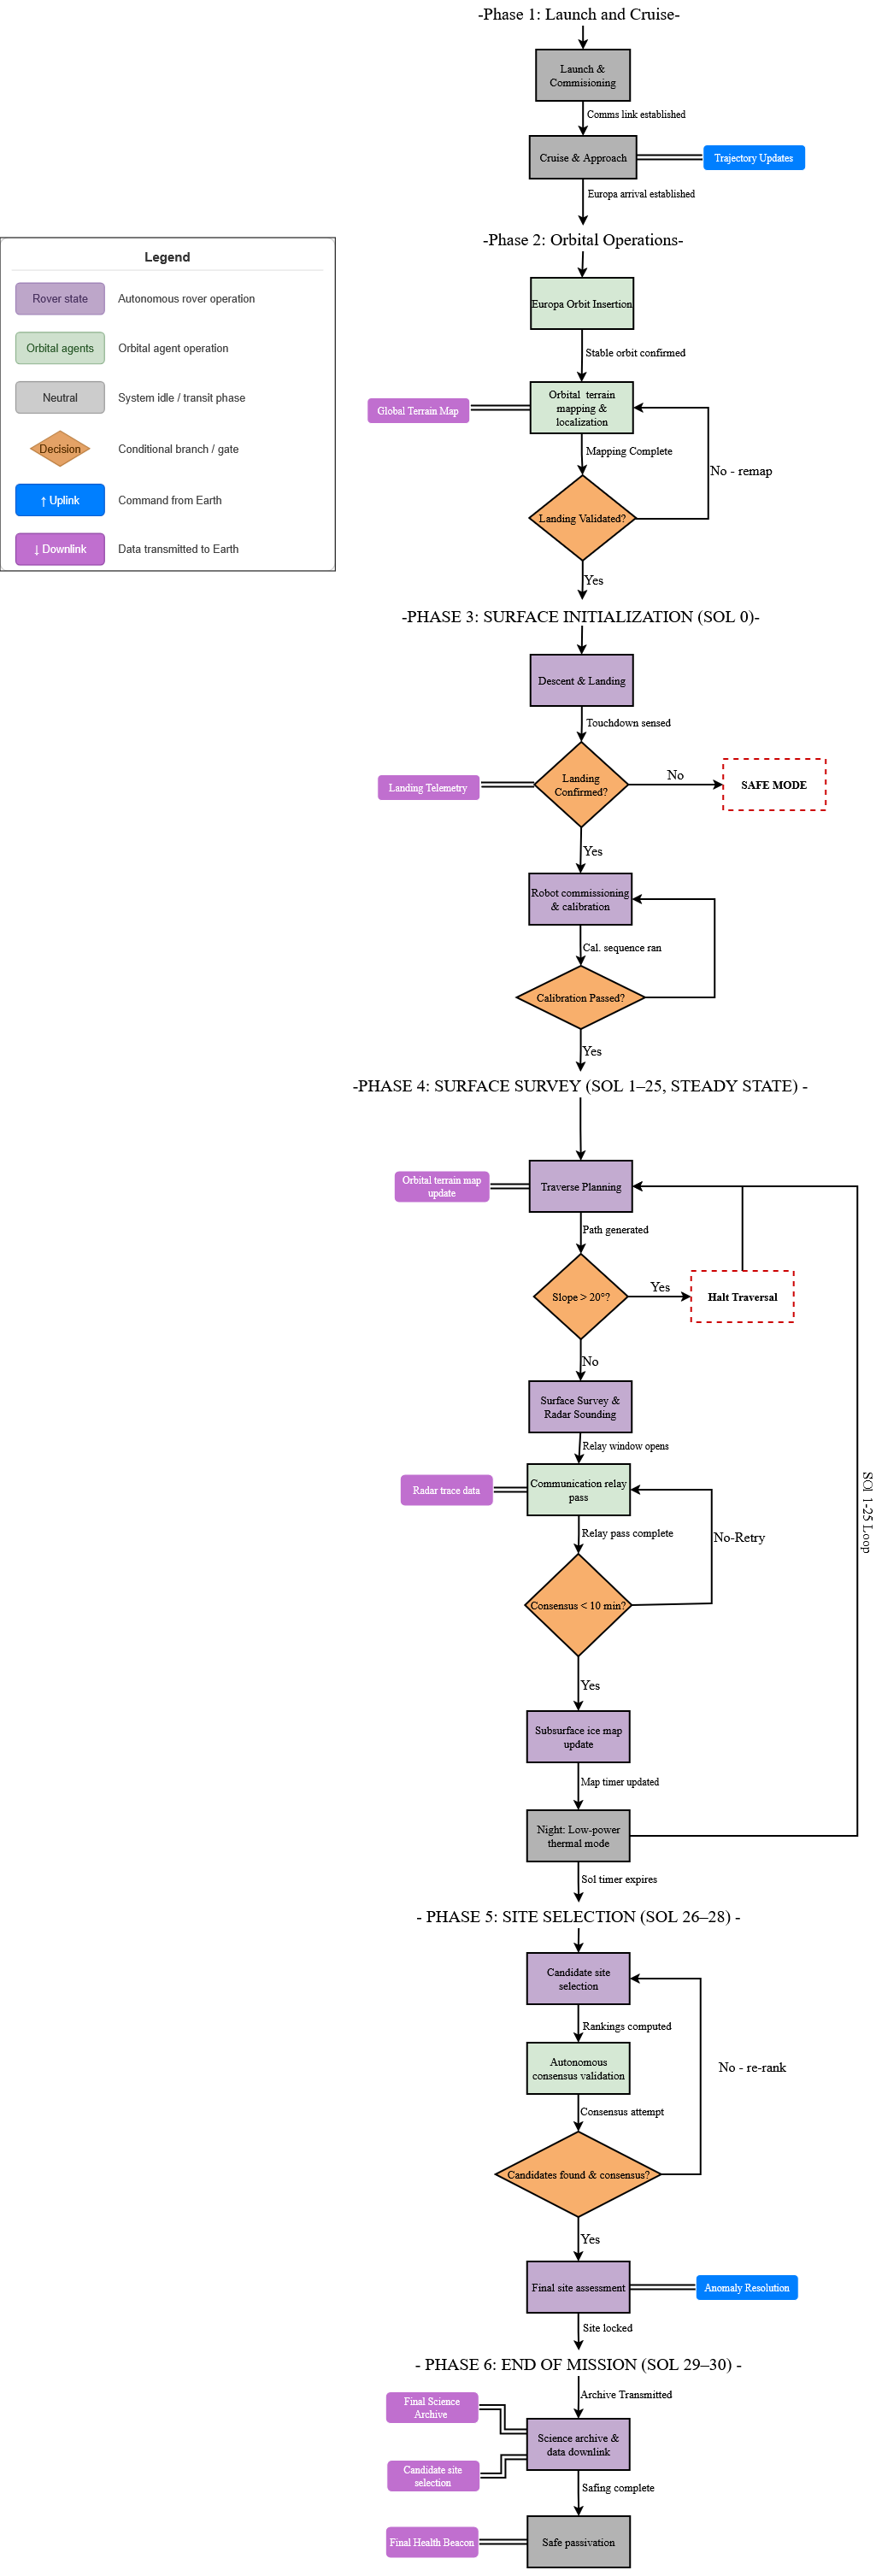
\includegraphics[width=0.55\textwidth]{figures/conops_state_flow.png}
    \caption{Flight-software / ConOps state flow across all six mission phases, with rover-state,
    orbital-agent, decision, uplink, and downlink blocks distinguished per the figure legend.}
    \label{fig:conops-state-flow}
\end{figure}

% ====================================================
% 5. PAYLOAD-DRIVEN DESIGN
% ====================================================
\section{Payload-Driven Design}

\subsection{Key Payload Description}

\textbf{Payload: REASON (Radar for Europa Assessment and Sounding: Ocean to
Near-surface)}

REASON is a dual-frequency ice-penetrating radar sounder currently flying aboard NASA's Europa
Clipper spacecraft. The instrument was developed by researchers at the University of Texas
Institute for Geophysics and fabricated by JPL, and it launched on October 14, 2024 atop a
SpaceX Falcon Heavy rocket bound for Europa~\cite{utigReason}. REASON operates at two frequency
bands simultaneously, allowing it to distinguish between near-surface structure and deep basal
reflections, a capability no previous Europa-targeted instrument has demonstrated~\cite{jplEuropaClipper}.
The instrument is flight-proven hardware with full mission-level heritage, placing it at TRL~9.

Europa Clipper carries REASON as part of a flyby science campaign: the spacecraft loops past
Europa roughly 50 times, collecting wide-swath regional maps of the ice shell from
altitude~\cite{wikiEuropaClipper}. This mission seeks to address what Clipper does not cover:
surface-level, high-resolution traverse profiling targeted at a specific candidate cryobot
insertion site. There is no rover, no in-situ localization, and no onboard site-selection logic
on Clipper, and the orbital geometry limits any single flyby to a brief snapshot rather than a
continuous along-track profile. This mission is essentially a continuation of Clipper: a surface
rover carrying an adapted REASON-heritage sounder drives a continuous traverse, building a
spatially registered subsurface map at $100$~m resolution or better, and autonomously flags the
thinnest viable ice for a future cryobot deployment.

REASON measures four primary parameters. Two-Way Travel Time (ns) is the elapsed time between
the transmitted pulse and the received basal reflection, and serves as the raw measurement.
Signal Amplitude (dB) captures the strength of the return from the ice-ocean interface; echoes
that fall into the noise floor are flagged to prevent false positives in site selection. Bulk Ice
Dielectric Permittivity (dimensionless) is estimated from the sounding's travel characteristics
($\varepsilon_r \approx 3.15$ for pure water ice), with deviations flagging brine pockets or
structural impurities. Finally, Derived Ice Shell Thickness (m) is computed autonomously onboard
using $d = c \cdot t\,/\,(2\sqrt{\varepsilon_r})$, where $c$ is the speed of light.

There are two crucial users of REASON's data. The onboard autonomous planning algorithm is the
real-time consumer: it continuously processes daily trace summaries to locate viable cryobot
deployment sites (ice thickness $<5$~km, surface slope $<20^\circ$, roughness index $<0.7$) and
issues a deployment trigger without human intervention when conditions are satisfied.
Earth-bound planetary scientists form the long-term consumer base: the full downlinked dataset
provides a high-resolution, spatially registered along-track profile of Europa's ice shell that
can be used to model global habitability, constrain ocean-access scenarios, and plan future
deep-subsurface entry missions.

\subsection{Payload Requirements}

The payload imposes concrete, traceable requirements on every other subsystem. Pointing:
REQ.03.02 requires the antenna boresight to stay within $\pm 5^\circ$ of nadir during active
sounding, forcing the rover to halt traversal whenever surface slope exceeds $20^\circ$; this
requirement is carried by Structures (antenna mast/mounting geometry) and Mobility
(slope-triggered halt logic). Power: REQ.03.03 requires a dedicated peak power allocation for
radar transmission pulses and commands drive-motor shutdown during each sounding window, since
the RTG's fixed continuous output cannot support simultaneous driving and sounding without
risking under-powering the radar pulse. Data handling: REQ.03.04 requires the CDH subsystem to
retain a minimum of 7 sols of uncompressed radar trace data and apply lossless compression at a
minimum $2{:}1$ ratio before inter-agent relay transmission, since raw science data accumulates
faster than the non-deterministic Earth relay link can clear it. Thermal: REQ.05.01 requires the
radar electronics (and all avionics) to stay within $0$--$40^\circ$C during active operations and
above $-20^\circ$C in night survival mode. Together these four requirements are why the payload,
rather than a generic bus design, drove the rover's mobility cadence (Section~7.7), power
budgeting (Section~7.4), onboard storage strategy (Section~6), and thermal architecture
(Section~7.5).

% ====================================================
% 6. DATA STRATEGY AND DELIVERABLES
% ====================================================
\section{Data Strategy and Deliverables}

\subsection{Data Product Table}

\textbf{Mission Objective:} Autonomously characterize Europa's ice shell thickness
along a surface traverse and identify an optimal cryobot insertion site without real-time Earth
support (REQ.03.01: ground-penetrating radar sounder resolves ice thickness to $\pm 10\%$ for
depths of 1--30~km at $\geq 100$~m along-track spatial resolution).

The data product is organized into four sheets so the dataset stays clear and usable.
Table~\ref{tab:data-sheets} summarizes each; full field-by-field definitions live in the source
2.1 Data Product deliverable.

\begin{table}[H]
\centering
\small
\begin{tabular}{p{2.6cm}p{5.5cm}p{4.7cm}}
\toprule
\textbf{Sheet} & \textbf{Key Fields (units)} & \textbf{Intended Consumers} \\
\midrule
Radar\_Traces & Trace ID, sol, along-track position (m), two-way travel time (ns), amplitude
(dB), permittivity (--), derived ice thickness (m), quality flag & Onboard site-selection
algorithm (real time); planetary scientists (post-mission) \\
Localization\_Log & Position X/Y (m, local ENU), heading (deg), $1\sigma$ uncertainty (m),
REQ.02.01 error flag & GNC/onboard planner; mission operations engineers \\
Terrain\_and\_Health & Surface slope (deg), roughness index (0--1), surface temperature (K),
accumulated TID (krad), radar noise floor (dB), inter-agent packet loss (\%), per-trace quality
flag & Onboard hazard/site filter; systems engineers monitoring health trends \\
Daily Summary & Traverse distance/sol (m), valid trace count, minimum ice thickness/sol (m),
candidate site count, mean consensus convergence time (min) & Mission planners (per-sol
go/no-go); operations team \\
\bottomrule
\end{tabular}
\caption{Data product sheets, key fields, and intended consumers.}
\label{tab:data-sheets}
\end{table}

Each data category maps to a specific requirement. The radar sounder returns are the direct
measurement required by REQ.03.01; without travel time and permittivity there is no thickness
inversion and no subsurface map. The localization log is required by REQ.02.01: each trace must
be placed within $\pm 0.5$~m to produce a spatially accurate map rather than an unordered list of
depth readings. Terrain context drives the site-selection filter, where slope and roughness
constrain physical accessibility independent of ice thickness. System health data is required by
REQ.01.02 and REQ.04.01: elevated TID can degrade radar performance, and packet loss above
$30\%$ directly stresses the consensus convergence bound. The main known limitation is
permittivity estimation uncertainty when brine inclusions or heterogeneous layering are present
(RISK-05); brine lenses increase local permittivity and can cause the thickness algorithm to
underestimate depth to the basal interface. The \texttt{CLUTTER} quality flag mitigates this by
excluding affected traces from site selection, but does not resolve the ambiguity without a
secondary instrument.

\subsection{Example Output}

On Sol~1 at $94.4$~s elapsed mission time (trace \texttt{TR-0001}), REASON recorded a two-way
travel time of $21{,}647.3$~ns, a return amplitude of $-41.62$~dB, a bulk ice permittivity of
$3.06$, and a derived ice shell thickness of $1{,}855.5$~m at rover position ($93.8$~m east,
$-7.1$~m north), with an accumulated total ionizing dose of $0.542$~krad and the record flagged
as \texttt{NOMINAL}. Tables~\ref{tab:sample-record} and~\ref{tab:sample-record-2} present this
trace together with the following 19 consecutive Sol-1 traces, exported directly from the
\textit{Data Product Space Robotics} spreadsheet (Radar\_Traces sheet, rows \texttt{TR-0001}
through \texttt{TR-0020}); four of the twenty are flagged \texttt{NOISE\_FLOOR} or
\texttt{CLUTTER} and correctly excluded from site-selection logic per Section~6.1.

\begin{table}[H]
\centering
\footnotesize
\begin{tabular}{lrrrrrr}
\toprule
Trace ID & Sol & Pos.\ E (m) & Pos.\ N (m) & TWT (ns) & Ampl.\ (dB) & $\varepsilon_r$ \\
\midrule
TR-0001 & 1 & 93.8 & $-7.1$ & 21{,}647.3 & $-41.62$ & 3.06 \\
TR-0002 & 1 & 185.5 & $-3.2$ & 169{,}839.5 & $-45.53$ & 3.10 \\
TR-0003 & 1 & 296.4 & 11.4 & 164{,}535.9 & $-25.34$ & 3.19 \\
TR-0004 & 1 & 382.9 & 7.0 & 131{,}950.8 & $-31.93$ & 3.34 \\
TR-0005 & 1 & 484.3 & $-0.6$ & 95{,}357.8 & $-49.20$ & 3.46 \\
TR-0006 & 1 & 577.3 & 7.4 & 23{,}845.1 & $-27.13$ & 3.40 \\
TR-0007 & 1 & 693.8 & 9.4 & 140{,}352.9 & $-51.49$ & 3.25 \\
TR-0008 & 1 & 779.5 & $-1.4$ & 145{,}118.1 & $-38.44$ & 3.37 \\
TR-0009 & 1 & 874.0 & 13.5 & 38{,}346.4 & $-40.26$ & 3.38 \\
TR-0010 & 1 & 960.4 & 18.9 & 118{,}968.0 & $-44.61$ & 3.30 \\
TR-0011 & 1 & 1{,}062.5 & 32.2 & 133{,}729.9 & $-55.42$ & 3.44 \\
TR-0012 & 1 & 1{,}156.1 & 26.0 & 41{,}835.8 & $-59.87$ & 3.36 \\
TR-0013 & 1 & 1{,}266.6 & 26.3 & 32{,}728.3 & $-34.99$ & 3.42 \\
TR-0014 & 1 & 1{,}361.5 & 16.1 & 181{,}816.0 & $-23.10$ & 3.46 \\
TR-0015 & 1 & 1{,}446.0 & 12.0 & 187{,}416.6 & $-27.73$ & 3.12 \\
TR-0016 & 1 & 1{,}529.2 & 18.9 & 157{,}620.1 & $-20.88$ & 3.27 \\
TR-0017 & 1 & 1{,}647.0 & 8.9 & 106{,}870.6 & $-35.74$ & 3.48 \\
TR-0018 & 1 & 1{,}754.6 & 15.3 & 84{,}222.6 & $-33.13$ & 3.19 \\
TR-0019 & 1 & 1{,}844.6 & 2.2 & 17{,}702.0 & $-37.84$ & 3.29 \\
TR-0020 & 1 & 1{,}926.9 & $-10.8$ & 19{,}528.7 & $-46.78$ & 3.26 \\
\bottomrule
\end{tabular}
\caption{Radar\_Traces sample export, Sol 1, traces TR-0001--TR-0020: position and raw sounding
returns.}
\label{tab:sample-record}
\end{table}

\begin{table}[H]
\centering
\footnotesize
\begin{tabular}{lrrl}
\toprule
Trace ID & Thickness (m) & TID (krad) & Flag \\
\midrule
TR-0001 & 1{,}855.5 & 0.542 & NOMINAL \\
TR-0002 & 14{,}478.5 & 0.577 & NOMINAL \\
TR-0003 & 13{,}818.1 & 0.735 & NOMINAL \\
TR-0004 & 10{,}827.1 & 0.817 & NOISE\_FLOOR \\
TR-0005 & 7{,}686.7 & 0.999 & NOMINAL \\
TR-0006 & 1{,}939.1 & 1.09 & NOMINAL \\
TR-0007 & 11{,}678.8 & 1.258 & NOMINAL \\
TR-0008 & 11{,}851.5 & 1.333 & NOMINAL \\
TR-0009 & 3{,}129.6 & 1.496 & NOMINAL \\
TR-0010 & 9{,}826.6 & 1.577 & CLUTTER \\
TR-0011 & 10{,}811.6 & 1.725 & NOMINAL \\
TR-0012 & 3{,}423.0 & 1.842 & NOMINAL \\
TR-0013 & 2{,}654.3 & 1.941 & NOMINAL \\
TR-0014 & 14{,}663.4 & 2.07 & NOMINAL \\
TR-0015 & 15{,}916.3 & 2.154 & NOMINAL \\
TR-0016 & 13{,}081.8 & 2.263 & CLUTTER \\
TR-0017 & 8{,}590.6 & 2.463 & CLUTTER \\
TR-0018 & 7{,}077.0 & 2.58 & NOMINAL \\
TR-0019 & 1{,}463.0 & 2.611 & NOMINAL \\
TR-0020 & 1{,}623.1 & 2.758 & NOMINAL \\
\bottomrule
\end{tabular}
\caption{Radar\_Traces sample export, Sol 1, traces TR-0001--TR-0020: derived ice thickness,
accumulated dose, and quality flag.}
\label{tab:sample-record-2}
\end{table}

Table~\ref{tab:sample-daily} exports both rows currently populated in the Daily\_Summary sheet
(Sol 1--2); the source spreadsheet has not yet been extended past Sol 2, so this is the complete
Daily\_Summary export available rather than an arbitrary 2-row excerpt.

\begin{table}[H]
\centering
\footnotesize
\begin{tabular}{rrrrrrrr}
\toprule
Sol & Traverse (m) & Valid & Bad & Min.\ Thickness (m) & Cand.\ Sites & Pkt.\ Loss (\%) &
Consensus (min) \\
\midrule
1 & 1{,}841.6 & 16 & 4 & 7{,}754.3 & 4 & 19.845 & 5.969 \\
2 & 1{,}804.8 & 16 & 4 & 9{,}750.0 & 1 & 19.795 & 5.959 \\
\bottomrule
\end{tabular}
\caption{Daily\_Summary sample export, Sol 1--2 (complete export of the sheet's current
contents).}
\label{tab:sample-daily}
\end{table}

% ====================================================
% 7. SYSTEM AND SUBSYSTEM DESIGNS
% ====================================================
\section{System and Subsystem Designs}

\subsection{Functional \& Nonfunctional Requirements}

Table~\ref{tab:functional} and Table~\ref{tab:nonfunctional} highlight five functional and five
nonfunctional requirements drawn from the master requirements set (Appendix~B has the complete
REQ.01.01--REQ.12.04 list with sources, subsystem ownership, and V\&V plans).

\begin{table}[H]
\centering
\small
\begin{tabular}{p{1.5cm}p{10.5cm}}
\toprule
\textbf{ID} & \textbf{Functional Requirement (what the system must do)} \\
\midrule
REQ.02.01 & Maintain localization accuracy no worse than $\pm 0.5$~m over any $50$~m traverse
segment in the absence of GPS. \\
REQ.03.01 & Resolve ice shell thickness to within $\pm 10\%$ for 1--30~km depths, at
$\geq 100$~m along-track resolution. \\
REQ.06.01 & Autonomously plan and execute $\geq 100$~m of surface traverse per sol, pausing at
$\leq 100$~m intervals for a radar sounding stop, and resume without ground uplink. \\
REQ.11.02 & Assess terrain out to $\geq 8$~m ahead of each drive arc and autonomously reject any
arc with a step $>0.20$~m, slope $>20^\circ$, or roughness $>0.7$. \\
REQ.11.04 & Halt traverse and enter a navigation hold whenever position uncertainty exceeds
$0.5$~m ($1\sigma$), and re-initialize via relay ranging plus map correlation. \\
\bottomrule
\end{tabular}
\caption{Representative functional requirements.}
\label{tab:functional}
\end{table}

\begin{table}[H]
\centering
\small
\begin{tabular}{p{1.5cm}p{10.5cm}}
\toprule
\textbf{ID} & \textbf{Nonfunctional Requirement (quality attribute / constraint)} \\
\midrule
REQ.01.01 & Operate fully autonomously for the entire surface mission without real-time Earth
uplinks (dependability / autonomy constraint). \\
REQ.01.02 & Survive and remain operational after $\geq 100$~krad total ionizing dose over the
mission lifetime (survivability). \\
REQ.05.01 & Maintain avionics/battery temperature within $0$--$40^\circ$C active, $>-20^\circ$C
night mode (environmental performance). \\
REQ.08.01 & Generate $\geq 110$~We (BOL) / $\geq 80$~We continuous via MMRTG-class RTG,
$\geq 1.9$~kWh usable per sol (capacity / performance). \\
REQ.10.03 & Close the rover--relay proximity link with $\geq 3$~dB margin over the required
$E_b/N_0$ at the $588$~km worst-case range (reliability / performance margin). \\
\bottomrule
\end{tabular}
\caption{Representative nonfunctional requirements.}
\label{tab:nonfunctional}
\end{table}

\subsection{Robot System Overview}

The system is a three-agent architecture: one surface rover and two orbital relay agents in
$200$~km circular Europa orbits. Broadly, the rover carries the science payload (REASON-heritage
GPR sounder) and mobility/GNC stack needed to physically reach and characterize a candidate
cryobot site; the orbital agents carry the terrain-mapping and communications-relay capability
the rover cannot provide for itself in a GPS-denied environment. Together they fulfill the
mission objective end to end: the orbiters find where it is safe to look, the rover determines
exactly how thick the ice is there, and the mesh network gets that answer back to Earth despite a
44-minute light delay.

Figure~\ref{fig:systems-overview} shows how the rover's subsystems interface with one another.
Power (RTG + battery packs) feeds every other subsystem over regulated $28$~V and $5$~V buses
through the PDU/EPS board; Thermal routes RTG waste heat to the radiators and survival heaters
and isolates the radiator loop with MLI and thermal switches; Structures provides the physical
mounting, radiation vault, and load path that the deployed legs, mast, and antenna assembly all
attach to; Avionics (the RAD750-class flight computer and I/O boards) hosts the GNC compute stack
and mediates between Comms, Payload, and Mobility; and Comms carries science data out over UHF
to the relay agents and commands back in, with an X-band link reserved as a low-rate,
direct-to-Earth contingency beacon. The GNC compute stack (visual odometry $\to$ navigation EKF
$\to$ hazard assessment $\to$ arc path planner $\to$ arc controller $\to$ mode manager/FDIR) is
the software layer that actually closes the loop between all of these physical interfaces every
drive arc.

\begin{figure}[H]
    \centering
    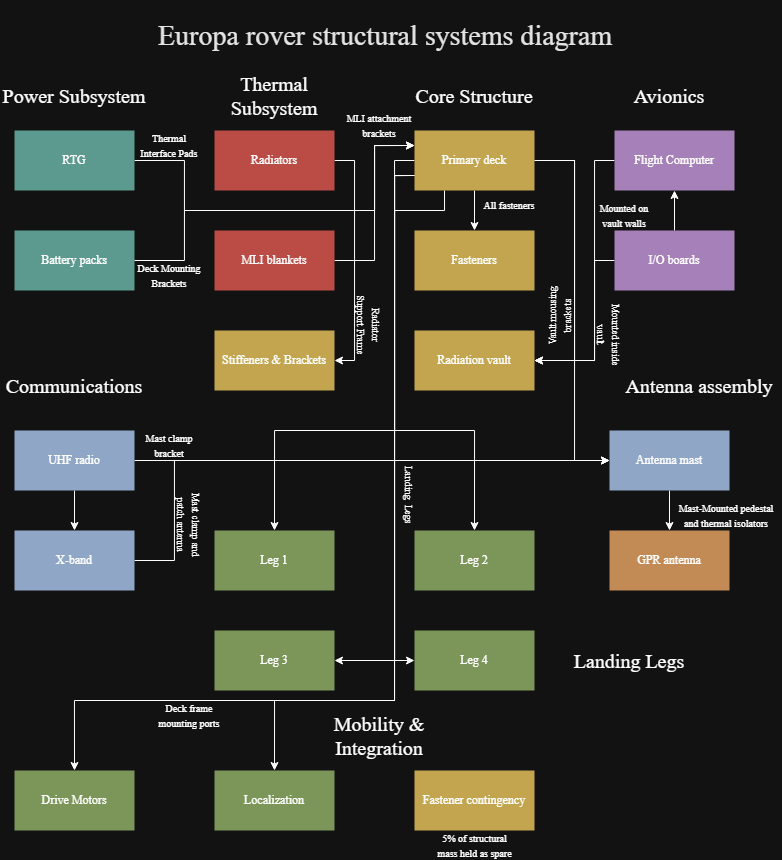
\includegraphics[width=0.95\textwidth]{figures/systems_diagram_overview.png}
    \caption{Rover systems diagram: subsystem-level interfaces across Power, Thermal, Core
    Structure, Avionics, Communications, Antenna Assembly, Landing Legs, and Mobility \&
    Integration.}
    \label{fig:systems-overview}
\end{figure}

\subsection{Structures and Mechanisms}

\subsubsection{Structural Requirements}
\begin{itemize}[leftmargin=*]
    \item \reqid{REQ.03.02}: Antenna boresight within $\pm 5^\circ$ of nadir during sounding;
    rover halts traversal above $20^\circ$ surface slope. (Structures, Science/Payload, Mobility)
    \item \reqid{REQ.07.01}: The rover chassis and landing leg structure shall accommodate
    vertical landing loads of $12g$ and lateral loads of $6g$ touchdown, with each leg sized to
    distribute peak contact forces across four footpads without permanent deformation or
    buckling. (Structures, Mobility, GNC)
    \item \reqid{REQ.07.02}: Primary equipment deck, fasteners, and all structural material
    shall remain within specification (yield strength, fatigue life) under sustained $90$~K
    cryogenic operation over the 30-sol mission lifetime. (Structures, Thermal, Power)
    \item \reqid{REQ.07.03}: The radiation shielding vault enclosing the flight computer and
    power distribution unit shall attenuate the Europa radiation environment to $\leq 1$~krad/sol
    at the electronics level, maintaining structural stiffness and mass allocation within the
    structures budget. (Structures, Power, Electronics, CDH)
\end{itemize}

\textbf{Resolved.} REQ.07.03's literal text previously allocated the radiation vault a
$28.5$~kg share of the structures budget against the $25.75$~kg Structure subsystem total in
Table~\ref{tab:mass-rollup}. The master spreadsheet now states $25.75$~kg consistently across
the requirement's ``shall'' statement, risk note, and verification plan (the latter also
specifying a $3.2$~kg allocation for the vault assembly itself within that total), matching the
mass budget; no $28.5$~kg figure remains anywhere in the requirement.

\subsubsection{Structural Sketch}
\begin{figure}[H]
    \centering
    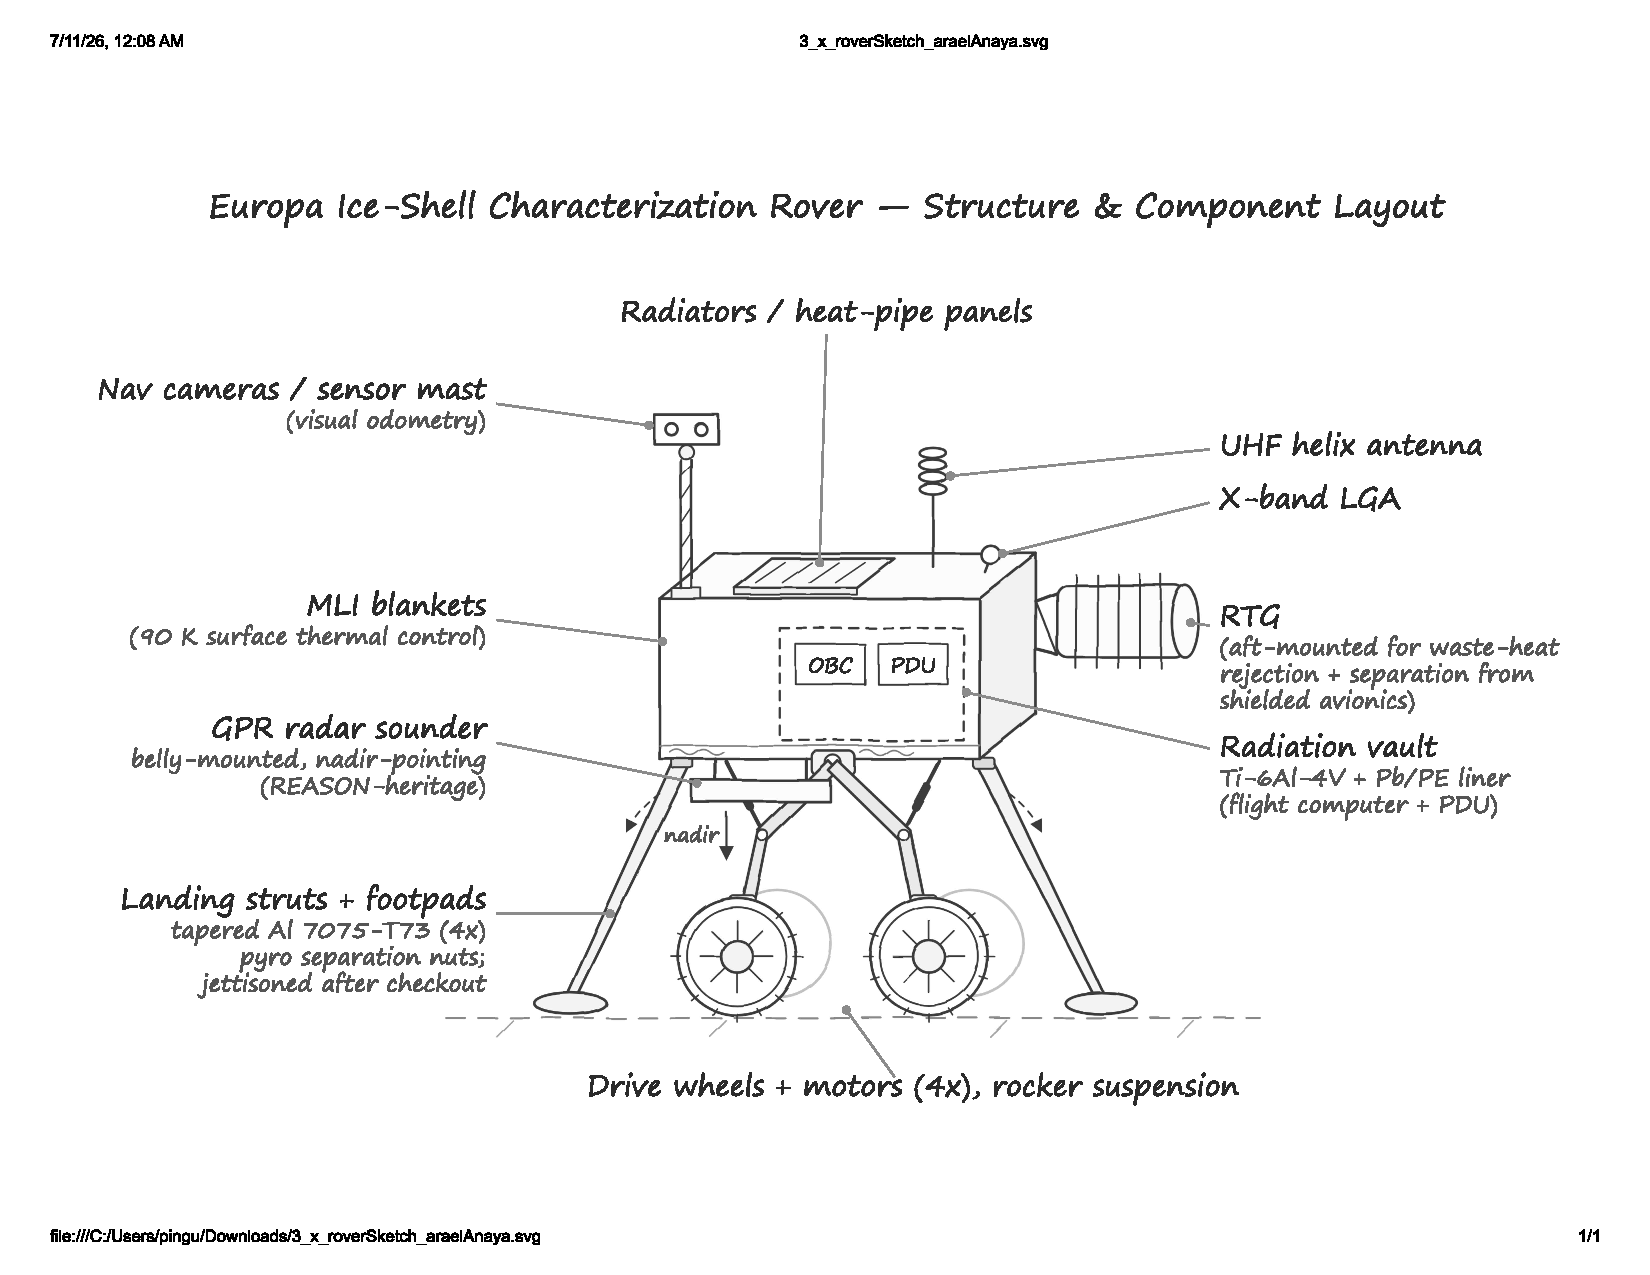
\includegraphics[width=0.85\textwidth]{figures/structures_sketch.pdf}
    \caption{Annotated structural sketch of the rover chassis, deck, radiation vault, antenna
    mast, and landing-leg arrangement.}
    \label{fig:structures-sketch}
\end{figure}

\subsubsection{Mass Budget}
Table~\ref{tab:mass-budget} reproduces the mass budget in full, including the Mobility line item
(Section~7.7, 3.6 Mobility Solution). Dry mass totals $134.90$~kg ($117.80$~kg core bus plus
$17.10$~kg of mobility hardware) against the $147.25$~kg contingency cap, leaving $12.35$~kg
($8.4\%$) of margin.

\begin{table}[H]
\centering
\footnotesize
\begin{tabular}{p{1.7cm}p{4.3cm}p{0.5cm}p{1.2cm}p{5.5cm}}
\toprule
\textbf{Subsystem} & \textbf{Component} & \textbf{Qty} & \textbf{Mass (kg)} & \textbf{Notes} \\
\midrule
Structure & Primary equipment decks/plates & 2 & 5.24 & Parametric sizing for avionics + GPR
antenna footprint \\
Structure & Landing legs (struts + footpads) & 4 & 10.36 & $2.59$~kg/leg, tolerates $<12g$
vertical / $6g$ lateral touchdown \\
Structure & Stiffeners/brackets/frames & 1 & 1.88 & Prevents deck deflection under landing loads \\
Structure & Fasteners \& support hardware & 1 & 1.42 & Cryogenic-rated titanium M5/M6 \\
Structure & Fastener contingency reserve & 1 & 0.73 & $5\%$ structural mass contingency \\
Structure & Antenna mast \& mounting bracket & 1 & 2.14 & GPR pedestal, Al tube + thermal
isolators for nadir pointing \\
Structure & Radiation shielding vault enclosure & 2 & 2.08 & Ti-6Al-4V; attenuates dose per
REQ.01.02 \\
Structure & Lead/polyethylene radiation liner & 1 & 1.56 & Selective shielding for flight
computer \\
Structure & Thermal interface pads & 2 & 0.34 & Minimizes thermal short through vault wall at
$90$~K \\
Thermal & MLI attachment structure & 1 & 1.44 & Brackets/clips for MLI retention + radiator
support \\
Thermal & Radiator support frame & 2 & 1.52 & Al tube frame, thermal decoupling \\
Thermal & MLI blankets & 1 & 6.32 & $0.35\ \mathrm{kg/m^2}$, $18.05\ \mathrm{m^2}$ equivalent
coverage \\
Thermal & Radiators / heat-pipe panels & 2 & 9.58 & $4.79$~kg/panel @ $6.0\ \mathrm{kg/m^2}$,
sized for $400$--$500$~W rejection \\
Power & Battery packs (12-hr survival) & 1 & 19.2 & $150$~Wh/kg $\times$ $16$~kg $+20\%$ margin \\
Power & PDU + high-current cabling & 1 & 4.68 & Heritage EPS scaling \\
Power & RTG & 1 & 28.0 & Main power source \\
Power & Heater & 1 & 2.86 & Heating unit \\
Comms & UHF radio + cabling & 2 & 1.83 & Heritage UHF radios, $1.5$--$2$~kg each \\
Comms & X-band transponder & 1 & 3.02 & DSN-compatible SDST heritage \\
Comms & Antennas (UHF helix / X-band LGA) & 1 & 0.86 & Short RF cabling \\
Avionics & Flight computer & 1 & 2.54 & OBC board + enclosure \\
Avionics & I/O / storage / interface boards & 1 & 1.52 & Logger + ADCs, includes enclosure \\
Payload & MEDA-class environment suite & 1 & 5.5 & Perseverance MEDA heritage, $\sim 17$~W op.
power \\
Software & Flight / GNC / FDIR & 0 & 0 & No physical mass; impacts OBC/EPS sizing only \\
Harness \& Integration & System harness / connectors / strain relief & 1 & 3.18 &
$2$--$3\%$ of dry mass \\
Mobility & Wheels, rocker suspension, drive motors, mast pan/tilt actuator (aggregate) & 1 &
17.10 & Per 3.6 Mobility Solution; not yet broken into individual component line items in the
source spreadsheet \\
\midrule
\multicolumn{4}{r}{\textbf{Dry Mass Total}} & \textbf{134.90 kg} \\
\multicolumn{4}{r}{\textbf{Remaining Margin vs.\ Cap}} & \textbf{12.35 kg (8.4\%)} \\
\multicolumn{4}{r}{\textbf{Mass Cap Limit}} & \textbf{147.25 kg} \\
\bottomrule
\end{tabular}
\caption{Rover mass budget by subsystem and component.}
\label{tab:mass-budget}
\end{table}

\begin{table}[H]
\centering
\small
\begin{tabular}{lrr}
\toprule
\textbf{Subsystem} & \textbf{Total Mass (kg)} & \textbf{\% Dry Mass} \\
\midrule
Structure & 25.75 & 19.09 \\
Thermal & 18.86 & 13.98 \\
Power & 54.74 & 40.58 \\
Comms & 5.71 & 4.23 \\
Avionics/OBC & 4.06 & 3.01 \\
Payload & 5.50 & 4.08 \\
Harness and Integration & 3.18 & 2.36 \\
Software & 0.00 & 0.00 \\
Mobility & 17.10 & 12.68 \\
\midrule
\textbf{Total} & \textbf{134.90} & \textbf{100.00} \\
\bottomrule
\end{tabular}
\caption{Mass budget rollup by subsystem.}
\label{tab:mass-rollup}
\end{table}

\textbf{Resolved.} The mobility solution's $17.1$~kg (Section~7.7: wheels, rocker suspension,
drive motors, mast pan/tilt actuator) is now carried as an explicit Mobility row in
Table~\ref{tab:mass-budget}/\ref{tab:mass-rollup} above, and the dry-mass total, rollup
percentages, and cap margin have been recomputed accordingly ($134.90$~kg vs.\ the $147.25$~kg
cap, $12.35$~kg/$8.4\%$ margin). The corresponding $3.5$~W is now carried as a Mobility row in
the power budget as well (Table~\ref{tab:power-budget}, Section~7.4), attributed to the mast
pan/tilt actuator drawing during the 1-hour Traverse Planning mode.

\subsubsection{Structures Trade Study}
\textbf{Study:} Analysis of Landing Leg Structure. Options were scored against six
pairwise-weighted criteria (Load Bearing Capability $0.25$, Mass per Leg $0.20$, Safety Margin
at Yield $0.25$, Thermal Conductivity $0.18$, Manufacturability \& TRL $0.25$, Cryogenic
Ductility $0.05$).

\begin{table}[H]
\centering
\small
\resizebox{\textwidth}{!}{%
\begin{tabular}{lccc}
\toprule
\textbf{Criterion (weight)} & \textbf{Tapered Strut Al 7075-T73} & \textbf{Cross-Braced Tube +
Diagonals} & \textbf{Ti-6Al-4V Folding Hinge (Hybrid)} \\
\midrule
Load Bearing (0.25) & 1.25 & 1.25 & 1.00 \\
Mass per Leg (0.20) & 0.80 & 0.60 & 0.60 \\
Safety Margin at Yield (0.25) & 1.25 & 1.25 & 1.00 \\
Thermal Conductivity (0.18) & 0.54 & 0.36 & 0.72 \\
Manufacturability \& TRL (0.25) & 1.25 & 0.75 & 0.50 \\
Cryogenic Ductility (0.05) & 0.20 & 0.25 & 0.15 \\
\midrule
\textbf{Total Score} & \textbf{5.29} & 4.46 & 3.97 \\
\bottomrule
\end{tabular}
}
\caption{Landing leg structure trade study.}
\label{tab:structures-trade}
\end{table}

\textbf{Winning option: Baseline tapered-strut Al 7075-T73 leg.} It matches the top
score on Load Bearing Capability and Safety Margin at Yield (both $5/5$) while separating itself
on Manufacturability \& TRL ($5/5$, off-the-shelf/heritage design, simple machining), which is
the largest single differentiator against the cross-braced and folding-hinge alternatives. This
is consistent with the $2.59$~kg/leg figure and material call-out already carried in the mass
budget (Table~\ref{tab:mass-budget}) and the tapered-strut geometry drawn in
Figure~\ref{fig:structures-sketch}.

\subsection{Electrical Power System}

\subsubsection{Power Requirements}
\begin{itemize}[leftmargin=*]
    \item \reqid{REQ.05.03}: Per-sol energy draw across all subsystems shall not exceed
    $90\%$ of the RTG's nominal daily energy output, reserving $\geq 10\%$ margin for anomaly
    response, heater activations, and unplanned relay passes. (Power, CDH, Thermal, Mobility)
    \item \reqid{REQ.08.01}: The power system shall generate $\geq 110$~We (BOL) via an
    MMRTG-class RTG and deliver $\geq 80$~We continuous upon Europa arrival, providing
    $\geq 1.9$~kWh usable energy per sol across the 30-sol surface mission. (Power, Thermal,
    System)
    \item \reqid{REQ.08.02}: Energy storage shall provide $\geq 2.4$~kWh usable capacity to
    (1)~load-level peak draws (drive motors, radar transmission, X-band downlink) beyond
    continuous RTG output, and (2)~sustain night-mode survival heating and critical avionics for
    $\geq 12$~hours, maintaining cell temperature above $-20^\circ$C per REQ.05.01. (Power,
    Thermal)
    \item \reqid{REQ.03.03}: Dedicated peak power allocation reserved for radar transmission
    pulses; drive motors commanded off during each active sounding window. (Science/Payload,
    Power, Mobility)
    \item \reqid{REQ.08.03}: The power distribution unit shall autonomously detect and
    isolate a faulted load bus within $100$~ms of overcurrent/undervoltage detection, maintain
    uninterrupted power to critical loads (flight computer, survival heaters, UHF radio), and
    log each fault event to non-volatile memory, without ground intervention. (Power, CDH,
    Electronics)
\end{itemize}

\subsubsection{Power Budget \& Profile}
Table~\ref{tab:power-budget} gives the per-component power budget; the RTG delivers a constant
$110$~W generated power baseline against which every mode is evaluated. Seven operating modes
were simulated across a 24-hour sol: Traverse Planning ($1$~hr), Traverse ($4$~hr), Radar
Sounding ($5$~hr), Comms Relay Pass ($1.5$~hr), Map Generation \& Consensus ($4.5$~hr), and Night
Low-Power ($8$~hr), summing to the full 24-hour cycle.

\begin{table}[H]
\centering
\footnotesize
\begin{tabular}{p{1.5cm}p{3.3cm}p{1.5cm}p{1.9cm}p{1.9cm}}
\toprule
\textbf{Subsystem} & \textbf{Component} & \textbf{Peak (W)} & \textbf{Avg (Wh/hr)} &
\textbf{Duration (h)} \\
\midrule
Payload & GPR Radar Sounder & 45 & 225.0 & 5.0 \\
EPS & Battery Packs & 0 & 0.0 & 24.0 \\
EPS & PDU (PCDU) & 12 & 288.0 & 24.0 \\
Mobility & Drive Motors (4x) & 84 & 336.0 & 4.0 \\
GNC & Flight Computer (OBC) & 18 & 432.0 & 24.0 \\
GNC & I/O \& Storage Boards & 6 & 96.0 & 16.0 \\
GNC & Nav Cameras & 4 & 20.0 & 5.0 \\
Thermal & Heaters & 40 & 320.0 & 8.0 \\
Thermal & Thermal Sensors & 0.5 & 12.0 & 24.0 \\
Comms & UHF Radio & 35 & 210.0 & 6.0 \\
Comms & X-band Transponder & 45 & 67.5 & 1.5 \\
Mobility & Mast Pan/Tilt Actuator & 3.5 & 3.5 & 1.0 \\
\midrule
\textbf{Total} & & & \textbf{2010.0 Wh/sol} & \\
\bottomrule
\end{tabular}
\caption{Power budget by component (peak draw and average energy consumption per sol). The
Mobility mast actuator (Section~7.7, 3.6 Mobility Solution) draws its $3.5$~W during Traverse
Planning, when the rover repositions the mast/antenna assembly ahead of the next drive arc.}
\label{tab:power-budget}
\end{table}

\begin{table}[H]
\centering
\small
\begin{tabular}{lccccccc}
\toprule
\textbf{Mode} & Traverse & Sounding & Comms Relay & Map Gen. & Traverse Plan. & Warm-Up & Night \\
\midrule
Avg.\ Power (W) & 124.5 & 81.5 & 116.5 & 71.5 & 44.0 & 121.5 & 70.5 \\
\bottomrule
\end{tabular}
\caption{Average power draw by operating mode.}
\label{tab:power-modes}
\end{table}

The battery (Max Charge $2400$~Wh, Min Safe Charge $480$~Wh) never approaches its
safety floor across the simulated 24-hour sol: lowest observed charge is $2342.1$~Wh (only
$\sim 58$~Wh, or $2.4\%$, below full), average power usage is $93.92$~W against $110$~W
generated, and highest charge/discharge rates are $69.5$~W/$14.5$~W respectively. This is
consistent with REQ.05.03's $90\%$-of-RTG-output cap with $10\%$ reserve: $93.92/110 = 85.4\%$,
inside the cap with margin to spare. (These daily-average and charge-profile figures predate the
Mobility mast actuator's $3.5$~Wh/sol addition above and have not been re-run in the source
mode-sequence simulation. As a first-order bound rather than a fresh simulation run: spreading the
actuator's $3.5$~Wh over the 24-hour sol raises average power usage to
$93.92 + 3.5/24 \approx 94.07$~W ($85.5\%$ of RTG output, still inside REQ.05.03's $90\%$ cap), and
the lowest observed charge falls by at most $3.5$~Wh in the worst case (to $\geq 2338.6$~Wh, i.e.\
$\leq 61.4$~Wh, or $\leq 2.6\%$, below full, still far above the $480$~Wh floor). Neither bound
changes the margin conclusion, but the exact
figures should still be regenerated by re-running the source mode-sequence simulation in the
master spreadsheet before they are cited as final.) Drive motors and the radar sounder are never
scheduled
concurrently in the mode matrix (REQ.03.03's stop-and-sound logic), and the flight computer,
PDU, and thermal sensors stay powered continuously across every mode as the ``always-on'' core
avionics load.

\textbf{Resolved.} The leftover satellite ground-pass boilerplate (``passes Hawaii roughly every
21 hours,'' ``over Hawaii for a maximum of about 7 minutes'') that previously appeared in the
Power Budget sheet's own annotations is now confined to the hidden raw-STK-data and legacy
mode-sequence tabs in the master spreadsheet; it no longer shows up in the visible sheets that
feed the exported Power Budget/Profile output or the totals above.

\begin{figure}[H]
    \centering
    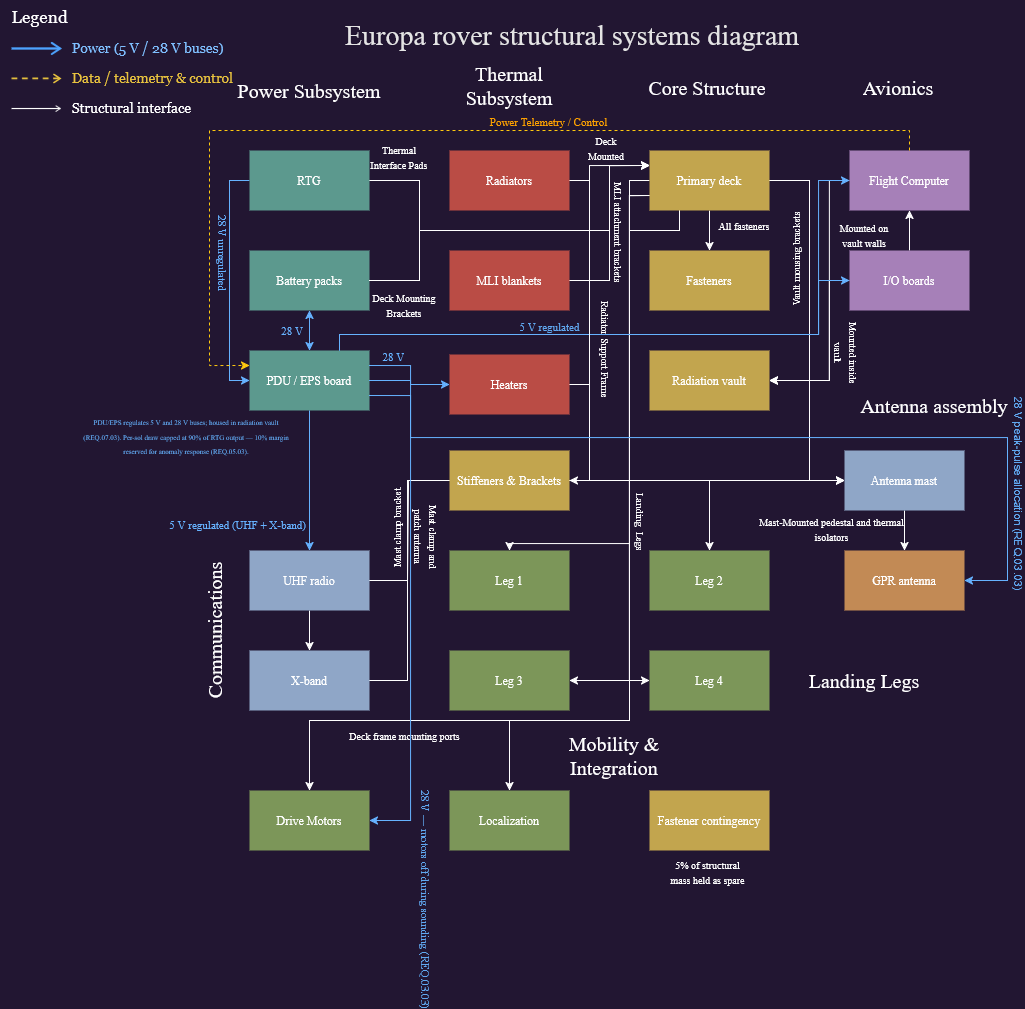
\includegraphics[width=0.95\textwidth]{figures/power_systems_diagram.png}
    \caption{Power systems diagram: RTG and battery packs feeding the PDU/EPS board over
    regulated $28$~V/$5$~V buses, with per-sol draw capped at $90\%$ of RTG output (REQ.05.03)
    and peak-pulse allocation reserved for the radar sounder (REQ.03.03).}
    \label{fig:power-diagram}
\end{figure}

\subsubsection{Power Trade Study}
\textbf{Study:} Analysis of Power Source. Options were scored against five
pairwise-weighted criteria (Mass $0.13$, Continuous Power $0.28$, Complexity/Operations $0.13$,
Radiation \& Cryo Robustness $0.25$, Availability/TRL $0.23$).

\begin{table}[H]
\centering
\small
\resizebox{\textwidth}{!}{%
\begin{tabular}{lccc}
\toprule
\textbf{Criterion (weight)} & \textbf{Solar Arrays + Li-ion} & \textbf{RTG} & \textbf{H\textsubscript{2}/O\textsubscript{2} Fuel Cells} \\
\midrule
Mass (0.13) & 0.25 & 0.38 & 0.13 \\
Continuous Power (0.28) & 0.28 & 1.38 & 0.55 \\
Complexity/Operations (0.13) & 0.25 & 0.63 & 0.25 \\
Radiation \& Cryo Robustness (0.25) & 0.50 & 1.25 & 0.75 \\
Availability/TRL (0.23) & 0.68 & 1.13 & 0.68 \\
\midrule
\textbf{Total Score} & 1.95 & \textbf{4.75} & 2.35 \\
\bottomrule
\end{tabular}
}
\caption{Power source trade study.}
\label{tab:power-trade}
\end{table}

\textbf{Winning option: RTG (radioisotope thermoelectric generator).} At $5.2$~AU,
solar irradiance has collapsed too far for arrays to deliver continuous power, and the RTG
scores a perfect $5/5$ on four of the five criteria (Continuous Power, Complexity/Operations,
Radiation \& Cryo Robustness, and Availability/TRL), losing only on raw mass (score $3/5$,
still the highest-weighted criterion it does not win). This selection is what sizes the $28$~kg
RTG line item in the mass budget (Table~\ref{tab:mass-budget}) and directly supports REQ.08.01's
$\geq 110$~We beginning-of-life requirement.

\subsection{Thermal Management}

\subsubsection{Thermal Requirements}
\begin{itemize}[leftmargin=*]
    \item \reqid{REQ.05.01}: Maintain avionics and battery cells within $0$--$40^\circ$C
    during active operations and above $-20^\circ$C during night-mode low-power management,
    using RTG-waste-heat-powered active heater elements. (Thermal, Power, Structures)
    \item \reqid{REQ.09.01}: Reject up to $500$~W of combined electronics dissipation and
    routed RTG waste heat through dedicated radiator panels, keeping the avionics vault below
    $40^\circ$C during peak daytime sounding/traverse operations. (Thermal, Electronics, Power,
    CDH)
    \item \reqid{REQ.09.02}: Preheat all drive-train actuators and deployment mechanisms
    above $-40^\circ$C before any commanded motion, completing cold-start warm-up within
    $60$~minutes of the $90$~K surface baseline. (Thermal, Mobility, Structures)
    \item \reqid{REQ.09.03}: Combine MLI with routed RTG waste heat to bound the
    equipment-enclosure heat leak such that supplemental electric survival heating does not
    exceed $50$~W and stays within the REQ.05.03 per-sol energy budget. (Thermal, Power,
    Structures)
\end{itemize}

\subsubsection{Heat Load Budget}
Table~\ref{tab:heat-loads} lists per-component power usage, efficiency, and resulting heat
generation. Aggregate power usage across all listed components is $289.5$~W at a blended
efficiency of $0.942$, for a total heat generation of $16.91$~W (this is the electronics
dissipation term; it excludes the RTG's own $\sim 2$~kW continuous thermal rejection, which is
routed separately as the primary survival heat source per REQ.09.03).

\begin{table}[H]
\centering
\footnotesize
\begin{tabular}{p{1.6cm}p{3.4cm}p{1.4cm}p{1.2cm}p{1.6cm}}
\toprule
\textbf{Board} & \textbf{Component} & \textbf{Power (W)} & \textbf{Eff.} & \textbf{Heat Gen.
(W)} \\
\midrule
Payload & GPR Radar Sounder (REASON-heritage) & 45 & 0.95 & 2.25 \\
EPS & Battery Packs & 0 & 1.00 & 0.00 \\
EPS & PDU (PCDU) & 12 & 0.93 & 0.84 \\
Mobility & Drive Motors (4x) & 84 & 0.90 & 8.40 \\
GNC & Flight Computer (OBC) & 18 & 0.95 & 0.90 \\
GNC & I/O \& Storage Boards & 6 & 0.95 & 0.30 \\
GNC & Nav Cameras (stereo VO) & 4 & 0.95 & 0.20 \\
Thermal & Heaters & 40 & 1.00 & 0.00 \\
Thermal & Thermal Sensors & 0.5 & 0.95 & 0.025 \\
Comms & UHF Radio (Electra-Lite heritage) & 35 & 0.95 & 1.75 \\
Comms & X-band Transponder & 45 & 0.95 & 2.25 \\
\midrule
\textbf{Total} & & \textbf{289.5} & \textbf{0.942} & \textbf{16.91} \\
\bottomrule
\end{tabular}
\caption{Heat load budget by component.}
\label{tab:heat-loads}
\end{table}

In addition to the equipment heat load above, a point-mass thermal equilibrium
analysis was performed for the avionics enclosure (area $0.12\ \mathrm{m^2}$, $\alpha = 0.20$,
$\varepsilon = 0.85$). The hot case ($Q_{int} = 20$~W, daytime operations) equilibrates at
$T_{hot} \approx 248$~K ($-25^\circ$C); the cold case ($Q_{int} = 5$~W, night survival)
equilibrates at $T_{cold} \approx 175$~K ($-98^\circ$C): a $\sim 73$~K swing. Unlike a
Mars-class mission, the problem on Europa is not rejecting heat but retaining it: solar
irradiance at $5.2$~AU collapses to $\sim 50\ \mathrm{W/m^2}$, so internal dissipation dominates
the energy balance, and even the operating case falls below the $\sim 253$~K ($-20^\circ$C) lower
bound for Li-ion battery charging. The survival case sits far outside any electronics or battery
limit and would freeze the system without intervention, which is exactly why MLI, routed RTG
waste heat, and controlled survival heaters (REQ.09.03) are required rather than optional.

\subsubsection{Thermal Trade Study}
\textbf{Study:} Analysis of Night Survival Thermal Architecture. Options were scored
$1$--$5$ against five pairwise-weighted criteria (Mass $0.13$, Power Demand $0.25$,
Complexity/Integration $0.13$, Radiation Durability $0.25$, Reliability/TRL $0.25$).

\begin{table}[H]
\centering
\small
\resizebox{\textwidth}{!}{%
\begin{tabular}{lccc}
\toprule
\textbf{Criterion (weight)} & \textbf{MLI + Heaters} & \textbf{Aerogel + Heaters} &
\textbf{PCM + Heat Pipes} \\
\midrule
Mass (0.13) & 0.52 & 0.52 & 0.26 \\
Power Demand (0.25) & 1.25 & 0.75 & 1.00 \\
Complexity/Integration (0.13) & 0.52 & 0.39 & 0.26 \\
Radiation Durability (0.25) & 1.25 & 0.75 & 0.75 \\
Reliability/TRL (0.25) & 1.25 & 0.75 & 0.50 \\
\midrule
\textbf{Total Score} & \textbf{4.79} & 3.16 & 2.77 \\
\bottomrule
\end{tabular}
}
\caption{Night-survival thermal architecture trade study.}
\label{tab:thermal-trade}
\end{table}

\textbf{Winning option: MLI and heaters} ($4.79$ vs.\ $3.16$ for aerogel + heaters and
$2.77$ for PCM with heat pipes). RTG waste heat ($\sim 1.9$~kW thermal) serves as the primary
survival heat source; MLI limits radiative loss so that supplemental electric survival heating
stays at or below $50$~W (REQ.09.03), keeping night thermal draw inside the per-sol energy budget
(REQ.05.03).

\begin{figure}[H]
    \centering
    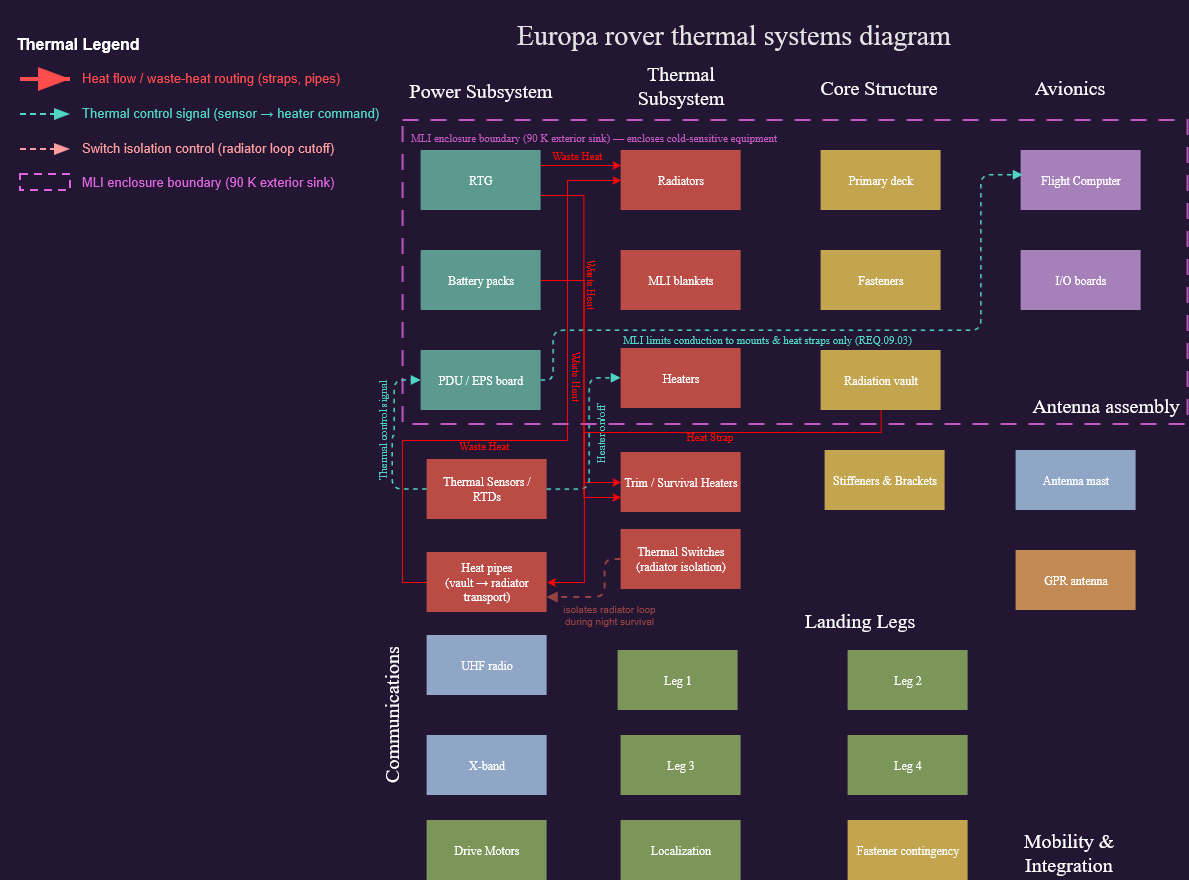
\includegraphics[width=0.95\textwidth]{figures/thermal_systems_diagram.png}
    \caption{Thermal systems diagram: RTG/heater waste-heat routing to radiators, MLI enclosure
    boundary, and radiator-loop isolation switches for night survival.}
    \label{fig:thermal-diagram}
\end{figure}

\subsection{Communications}

\subsubsection{Communications Requirements}
\begin{itemize}[leftmargin=*]
    \item \reqid{REQ.01.03}: Maintain $\geq 2$ active relay nodes at all times during surface
    operations. (System, COMMs)
    \item \reqid{REQ.04.01}: Inter-agent mesh network shall achieve terrain-map consensus
    within $\leq 10$~minutes under $\leq 30\%$ packet loss on any single link. (COMMs, CDH)
    \item \reqid{REQ.10.01}: Deliver $\geq 55$~MB/Earth-day compressed data at $\geq 128$~kbps
    return / $\geq 8$~kbps forward. (COMMs, CDH, Science/Payload, Power)
    \item \reqid{REQ.10.02}: Obtain $\geq 2$ usable relay contacts/sol totaling $\geq 90$~min
    above a $10^\circ$ elevation mask; end-to-end latency $\leq 26$~hours. (COMMs, CDH,
    Science/Payload, GNC)
    \item \reqid{REQ.10.03}: Close the proximity link with $\geq 3$~dB margin at the
    worst-case $588$~km slant range; retain an X-band DTE beacon $\geq 5$~bps as a relay-loss
    fallback. (COMMs, Power, Structures, CDH)
\end{itemize}

\subsubsection{Comm Architecture \& Assumptions}
The rover's next communication node is the nearer of the two orbital relay agents; the mission
does not route science data through a direct link to Earth in nominal operations. The link uses a
UHF proximity band on the CCSDS Proximity-1 return/forward pair: $401.6$~MHz return,
$437.1$~MHz forward, the same split flown by Electra and Electra-Lite on the Mars Relay Network.
Desired margin is $3$~dB above the $E_b/N_0$ required for a post-decoding bit error rate of
$10^{-6}$ (CCSDS turbo coding, rate $1/2$, threshold near $1.5$~dB, so the link must clear
$4.5$~dB total): a conservative cushion given that the relay's exact orbit geometry, the
rover's helix gain pattern, and Jupiter's synchrotron noise contribution are all still modeled
rather than measured. Worst-case geometry assumes both relays fly a $200$~km circular Europa
orbit; with a $10^\circ$ elevation mask, the slant range at the edge of a pass is $588$~km, and
every link budget term uses that worst case.

Rover transmit power is $5$~W RF into a $5.0$~dBi quadrifilar helix (near-hemispherical pattern,
so the rover can close a pass without pointing at anything); the relay carries $8$~W RF into a
$7.0$~dBi patch array, since its power budget has more slack. System noise temperature is
$3000$~K at the relay receiver and $4000$~K at the rover receiver: the number that most
separates a Europa proximity link from a Mars one, since at $400$~MHz the receiver picks up
galactic background noise on top of Jupiter's synchrotron emission. The return link runs
$128$~kbps (sized to clear $55$~MB in the $90$-minute relay window) and the forward link runs
$8$~kbps (commands only). Figure~\ref{fig:comms-architecture} shows the full data-flow
architecture from the payload through CDH, the modem/transceiver chain, the RF front end, and out
to the relay agents and, ultimately, the DSN.

\begin{figure}[H]
    \centering
    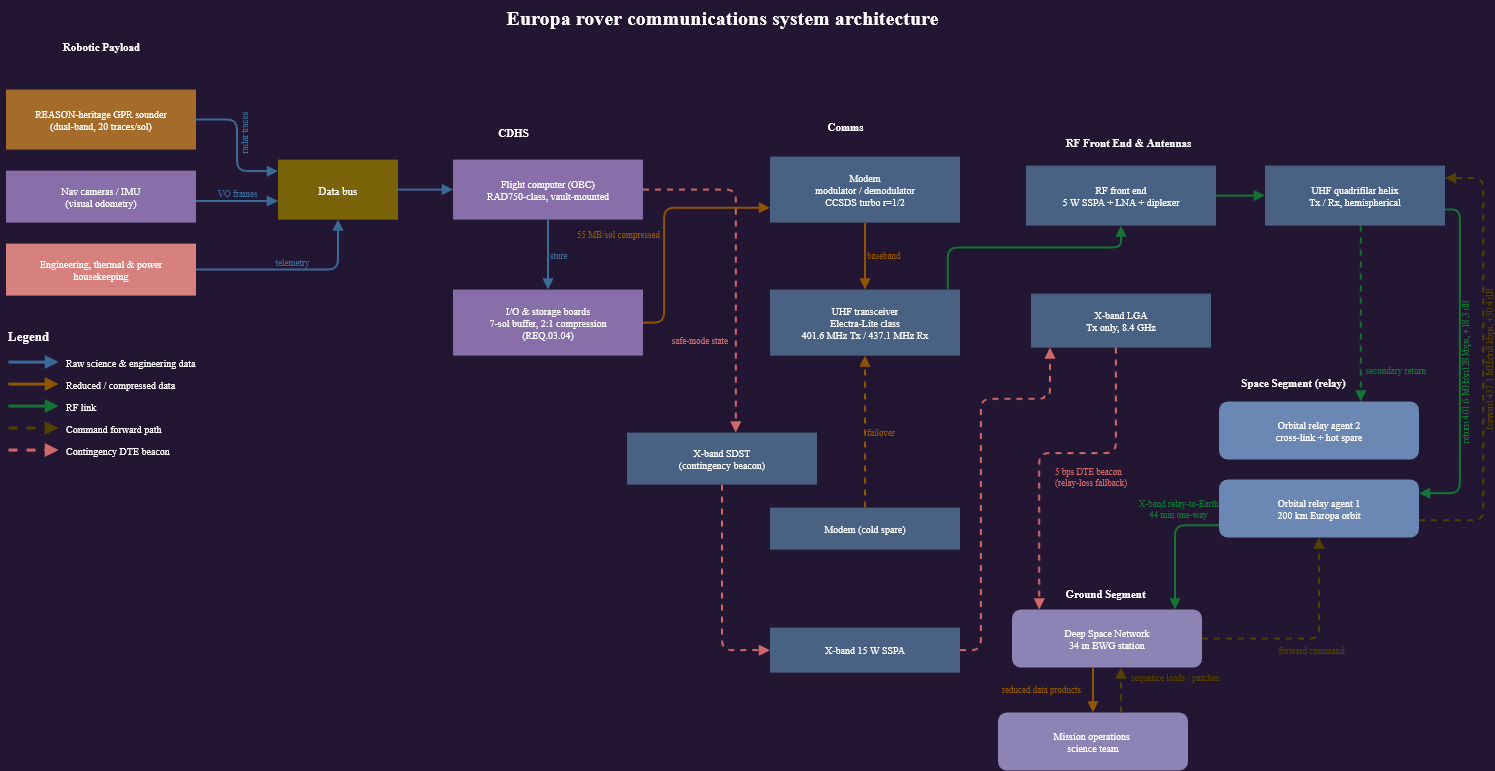
\includegraphics[width=0.95\textwidth]{figures/comms_architecture.png}
    \caption{Communications system architecture: data flow from payload/nav/health sources
    through CDH, comms, and the RF front end to the orbital relay agents and DSN ground segment.}
    \label{fig:comms-architecture}
\end{figure}

\subsubsection{Partial Link Budget}
Both directions close with wide margin: $18.3$~dB on the return (uplink, rover$\to$relay) and
$30.4$~dB on the forward (downlink, relay$\to$rover), against a $4.5$~dB requirement.
Table~\ref{tab:link-budget} breaks the return link down term by term.

\begin{table}[H]
\centering
\small
\begin{tabular}{lr}
\toprule
\textbf{Term} & \textbf{Value (dB)} \\
\midrule
$P_t$ ($5$~W) & $+6.99$ \\
$G_t$ (rover helix) & $+5.00$ \\
$G_r$ (relay patch array) & $+7.00$ \\
$L_a$ (polarization + plasma) & $-0.51$ \\
$L_l$ (line loss) & $-1.49$ \\
$\lambda^2$ & $-2.54$ \\
$(4\pi R)^2$ (space loss @ $588$~km) & $-137.37$ \\
$k$ & $+228.60$ \\
$T_s$ ($3000$~K) & $-34.77$ \\
$R_b$ ($128$~kbps) & $-51.07$ \\
\midrule
$E_b/N_0$ & $\mathbf{+19.84}$ \\
Margin over $1.5$~dB requirement & $\mathbf{+18.3}$ \\
\bottomrule
\end{tabular}
\caption{Return-link (rover-to-relay) budget, term by term.}
\label{tab:link-budget}
\end{table}

As a direct-to-Earth sanity check: the rover's X-band low-gain antenna against a DSN
$34$~m station closes at roughly $6.9$~bps at opposition ($4.2$~AU) and $3.2$~bps at conjunction
($6.2$~AU) while holding the same $4.5$~dB margin: enough for a state-of-health beacon, but a
single $55$~MB sol of science data would take over two years to clear at that rate. This is why
the relay architecture is foundational rather than a convenience (REQ.10.03's $5$~bps fallback
floor is set directly from this analysis).

\subsubsection{Communications Subsystem Diagram}
\begin{figure}[H]
    \centering
    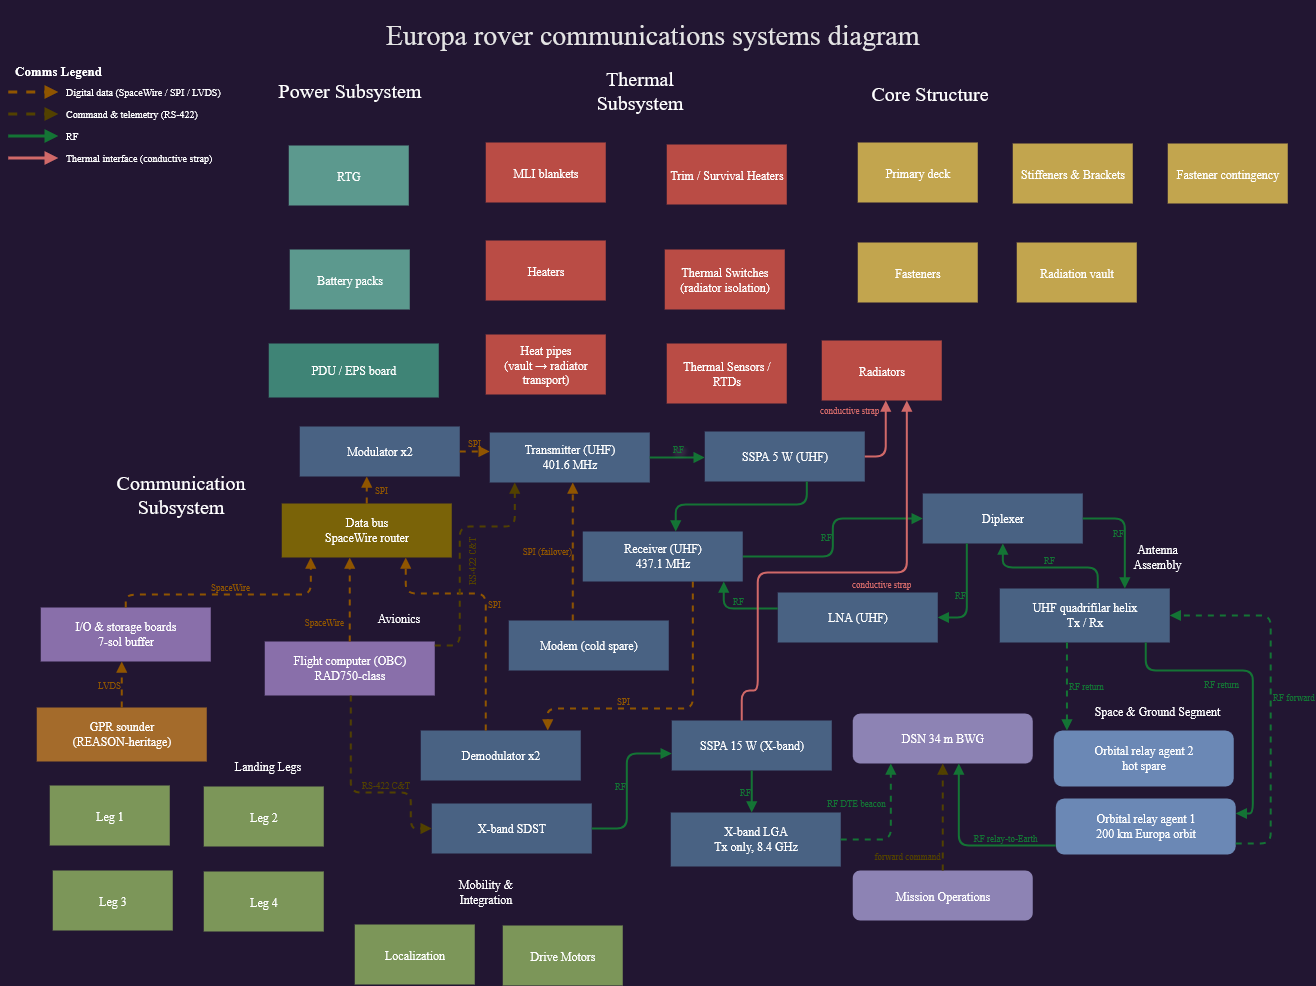
\includegraphics[width=0.95\textwidth]{figures/comms_systems_diagram.png}
    \caption{Communications systems diagram: modulator/transceiver chain, RF front end, and
    antenna assembly, with digital-data, command/telemetry, RF, and thermal-interface signal
    paths distinguished.}
    \label{fig:comms-systems}
\end{figure}

\subsubsection{Communications Trade Study}
\textbf{Study:} Analysis of Rover-to-Relay Proximity Link Configuration. Options were
scored against five pairwise-weighted criteria (Mass $0.13$, Power Demand $0.25$, Data Rate
Capability $0.25$, Pointing \& Ops Complexity $0.13$, Reliability/TRL $0.25$).

\begin{table}[H]
\centering
\small
\resizebox{\textwidth}{!}{%
\begin{tabular}{lccc}
\toprule
\textbf{Criterion (weight)} & \textbf{UHF Helix} & \textbf{S-band Patch} &
\textbf{X-band Gimballed HGA} \\
\midrule
Mass (0.13) & 0.65 & 0.52 & 0.26 \\
Power Demand (0.25) & 1.00 & 0.75 & 0.50 \\
Data Rate Capability (0.25) & 1.00 & 1.25 & 1.25 \\
Pointing \& Ops Complexity (0.13) & 0.65 & 0.52 & 0.13 \\
Reliability/TRL (0.25) & 1.25 & 0.75 & 0.50 \\
\midrule
\textbf{Total Score} & \textbf{4.55} & 3.79 & 2.64 \\
\bottomrule
\end{tabular}
}
\caption{Rover-to-relay proximity link configuration trade study.}
\label{tab:comms-trade}
\end{table}

\textbf{Winning option: UHF quadrifilar helix} ($401.6$/$437.1$~MHz). The X-band option
has the raw throughput but fails the other criteria: a two-axis gimbal is a moving mechanism that
has to survive $90$~K and $100$~krad, and it needs closed-loop tracking of a relay the rover
cannot see coming. S-band buys data rate the mission does not need, since the UHF return already
closes at $128$~kbps with $18.3$~dB of margin and is bounded by the transceiver's $2048$~kbps
ceiling rather than by RF. The helix is already in the mass budget at $0.86$~kg and carries TRL~9
through Electra and Electra-Lite heritage on exactly this kind of proximity link.

\subsection{GNC and Mobility}

\subsubsection{GNC Requirements}
\begin{itemize}[leftmargin=*]
    \item \reqid{REQ.11.01}: Determine attitude to $\pm 0.5^\circ$ ($3\sigma$) roll/pitch and
    heading to $\pm 0.25^\circ$ ($3\sigma$) at every sounding stop, propagating inertially
    between arcs $\leq 5$~m and taking an absolute heading fix from fine sun sensors at each arc
    end. (GNC, Mobility, Science/Payload, CDH)
    \item \reqid{REQ.11.02}: Assess terrain $\geq 8$~m ahead via stereo nav cameras before
    each drive arc; autonomously reject arcs with a step $>0.20$~m, slope $>20^\circ$, or
    roughness $>0.7$; stop within $0.25$~m of the assessed safe limit. (GNC, Mobility,
    Science/Payload, CDH)
    \item \reqid{REQ.11.03}: Follow the planned path with cross-track deviation $\leq 0.5$~m
    over a $50$~m segment and stop within $\pm 0.5$~m of each commanded waypoint, using
    differential drive with wheel slip estimated from the odometry/visual-odometry residual.
    (GNC, Mobility, Science/Payload)
    \item \reqid{REQ.11.04}: Halt and enter a navigation hold whenever $1\sigma$ position
    uncertainty exceeds $0.5$~m; re-initialize via two-way ranging to $\geq 2$ relay agents plus
    local/orbital terrain correlation; do not resume until uncertainty is restored below
    $0.5$~m. (GNC, COMMs, CDH, Mobility)
\end{itemize}

\subsubsection{Mobility Solution Sketch}
\textbf{Configuration: Four-Wheel Differential Drive on a Single-Pivot Rocker.} Four
independently driven wheels ride on a single-pivot rocker, with no steering actuators. The
chassis is the $0.90$~m $\times$ $0.60$~m equipment deck already carried in the mass budget, held
$0.35$~m above the surface so the belly-mounted sounder keeps its standoff. Wheelbase is
$0.70$~m and track is $0.80$~m; wheels are $0.32$~m in diameter, $0.20$~m wide, with a rigid
aluminum rim carrying 24 hardened cleats. Commanded speed is $2$~cm/s, driven in arcs no longer
than $5$~m.

Wheels were chosen over hopping or legged locomotion because the mission needs a spatially
continuous subsurface profile: REQ.03.01 calls for a radar trace every $100$~m or better along a
single transect, and every landing event in a hop or step creates a gap where the localization
solution has to start over. A hop that lands wrong on a $90$~K ice block can end the mission on
the spot, with no window for Earth to intervene given the $44$-minute one-way delay; a wheeled
rocker instead degrades slowly, bearing by bearing, over many sols: a failure mode better
suited to a mission with no recovery crew.

\begin{figure}[H]
    \centering
    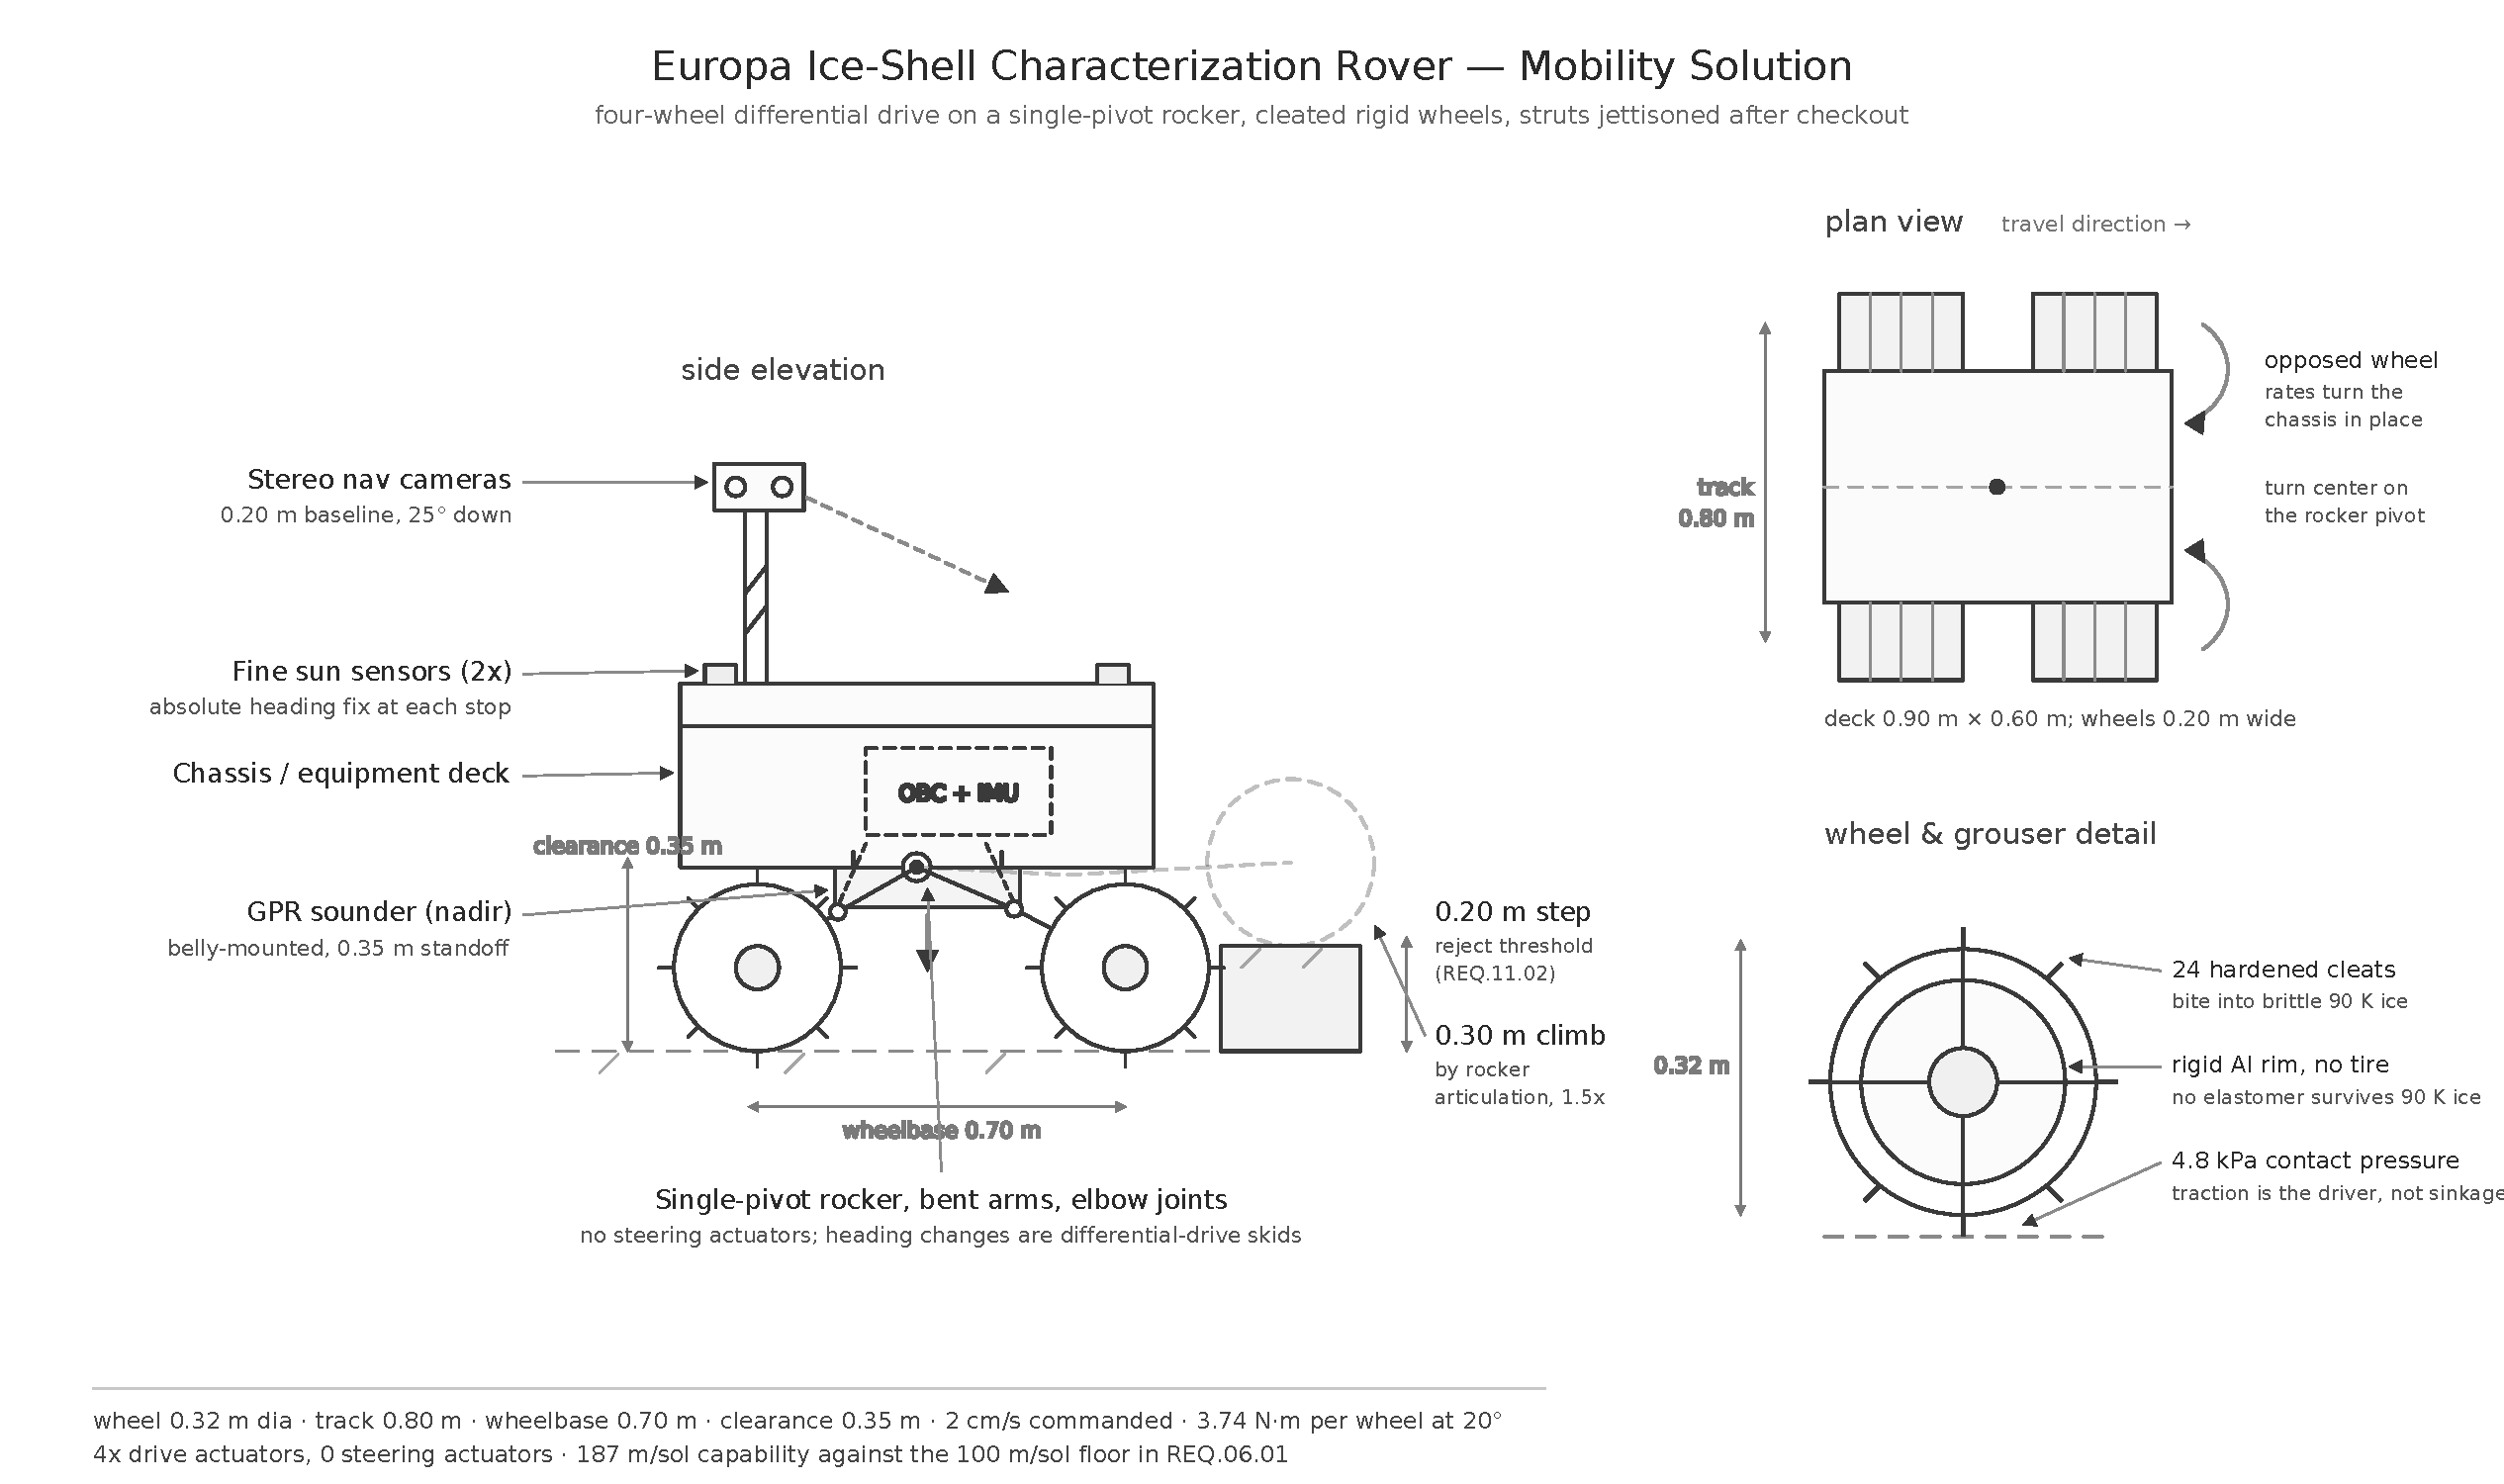
\includegraphics[width=0.95\textwidth]{figures/mobility_sketch.pdf}
    \caption{Mobility solution: side elevation, plan view, and wheel detail.}
    \label{fig:mobility-sketch}
\end{figure}

Steering is handled entirely by differential drive: opposing wheel rates rotate the chassis about
the rocker pivot, so every heading change is a deliberate skid across the ice. Skid steering
slips badly on hard ice ($\mu \approx 0.5$), so wheel odometry is dropped as a position source and
used instead as a slip observable: the residual between encoder counts and stereo visual
odometry becomes the slip estimate, the same approach the MER rovers used on Martian
sand~\cite{maimone}. Heading is re-anchored with an absolute sun-sensor fix at the end of every
$5$~m arc so error never integrates across a full traverse segment.

\subsubsection{Localization and Pointing Budget}
Table~\ref{tab:loc-budget} closes the $50$~m segment localization error budget: root-sum-square
of $0.46$~m against the $0.5$~m limit in REQ.02.01, an $8\%$ margin.

\begin{table}[H]
\centering
\small
\begin{tabular}{lc}
\toprule
\textbf{Error source over a 50~m segment} & \textbf{Contribution (m)} \\
\midrule
Visual odometry scale and feature residual & 0.30 \\
Heading knowledge ($0.271^\circ$) & 0.24 \\
Wheel slip on cleated water ice & 0.20 \\
Inter-agent range residual & 0.15 \\
\midrule
Root-sum-square & \textbf{0.46} \\
REQ.02.01 limit & 0.50 \\
\bottomrule
\end{tabular}
\caption{Localization error budget, one 50~m traverse segment.}
\label{tab:loc-budget}
\end{table}

In addition to this position-error rollup, the source pointing budget defines
per-component alignment requirements rather than a single combined pointing RSS: the GPR
antenna boresight must hold $\pm 5^\circ$ of nadir ($\pm 0.5^\circ$ stop-to-stop repeatability,
REQ.03.02); the fine sun sensor pair resolves the Sun vector to $\pm 0.1^\circ$, which folds into
a $\pm 0.25^\circ$ heading solution after ephemeris and mounting alignment error (REQ.11.01); and
the stereo nav camera boresight sits $25^\circ$ below the local horizontal with a $0.20$~m
step-detection capability at $8$~m range (REQ.11.02).

\subsubsection{GNC Trade Study}
\textbf{Study:} Analysis of the absolute heading reference for surface navigation.
Options were scored against five pairwise-weighted criteria (Mass $0.12$, Power Demand $0.23$,
Complexity/Cost $0.12$, Accuracy $0.30$, Environmental Tolerance $0.23$).

\begin{table}[H]
\centering
\small
\resizebox{\textwidth}{!}{%
\begin{tabular}{lccc}
\toprule
\textbf{Criterion (weight)} & \textbf{Fine Sun Sensor Pair} & \textbf{COTS Star Tracker} &
\textbf{FOG Gyrocompassing} \\
\midrule
Mass (0.12) & 0.60 & 0.48 & 0.24 \\
Power Demand (0.23) & 1.15 & 0.69 & 0.46 \\
Complexity/Cost (0.12) & 0.48 & 0.24 & 0.12 \\
Accuracy (0.30) & 1.20 & 1.50 & 0.90 \\
Environmental Tolerance (0.23) & 1.15 & 0.46 & 0.46 \\
\midrule
\textbf{Total Score} & \textbf{4.58} & 3.37 & 2.18 \\
\bottomrule
\end{tabular}
}
\caption{Absolute heading reference trade study.}
\label{tab:gnc-trade}
\end{table}

\textbf{Winning option: Fine sun sensor pair with onboard ephemeris.} The star tracker
wins on raw accuracy and loses everywhere else: its detector degrades measurably under the
Jovian dose, it needs a baffle against Jupiter (which subtends $\sim 11.8^\circ$ from the surface
and never sets on the sub-Jovian hemisphere), and it costs more than the rest of the GNC sensor
suite combined. Gyrocompassing is the interesting failure: a $0.01^\circ$/h FOG can in principle
find north off Europa's $4.22^\circ$/h rotation, but that signal is only $28\%$ of what the same
instrument would see on Earth, and the fiber coil and light source are not qualified at $90$~K or
$100$~krad. The sun sensor is the cheap answer: at $5.2$~AU the Sun delivers only
$50\ \mathrm{W/m^2}$, but its angular diameter collapses to $0.103^\circ$, so a photodiode sensor
is looking at a sharper point source than it would at Earth. Two of them cost $0.12$~kg and under
$1$~W, and Cassini flew the same class of sensor further out than Jupiter.

\begin{figure}[H]
    \centering
    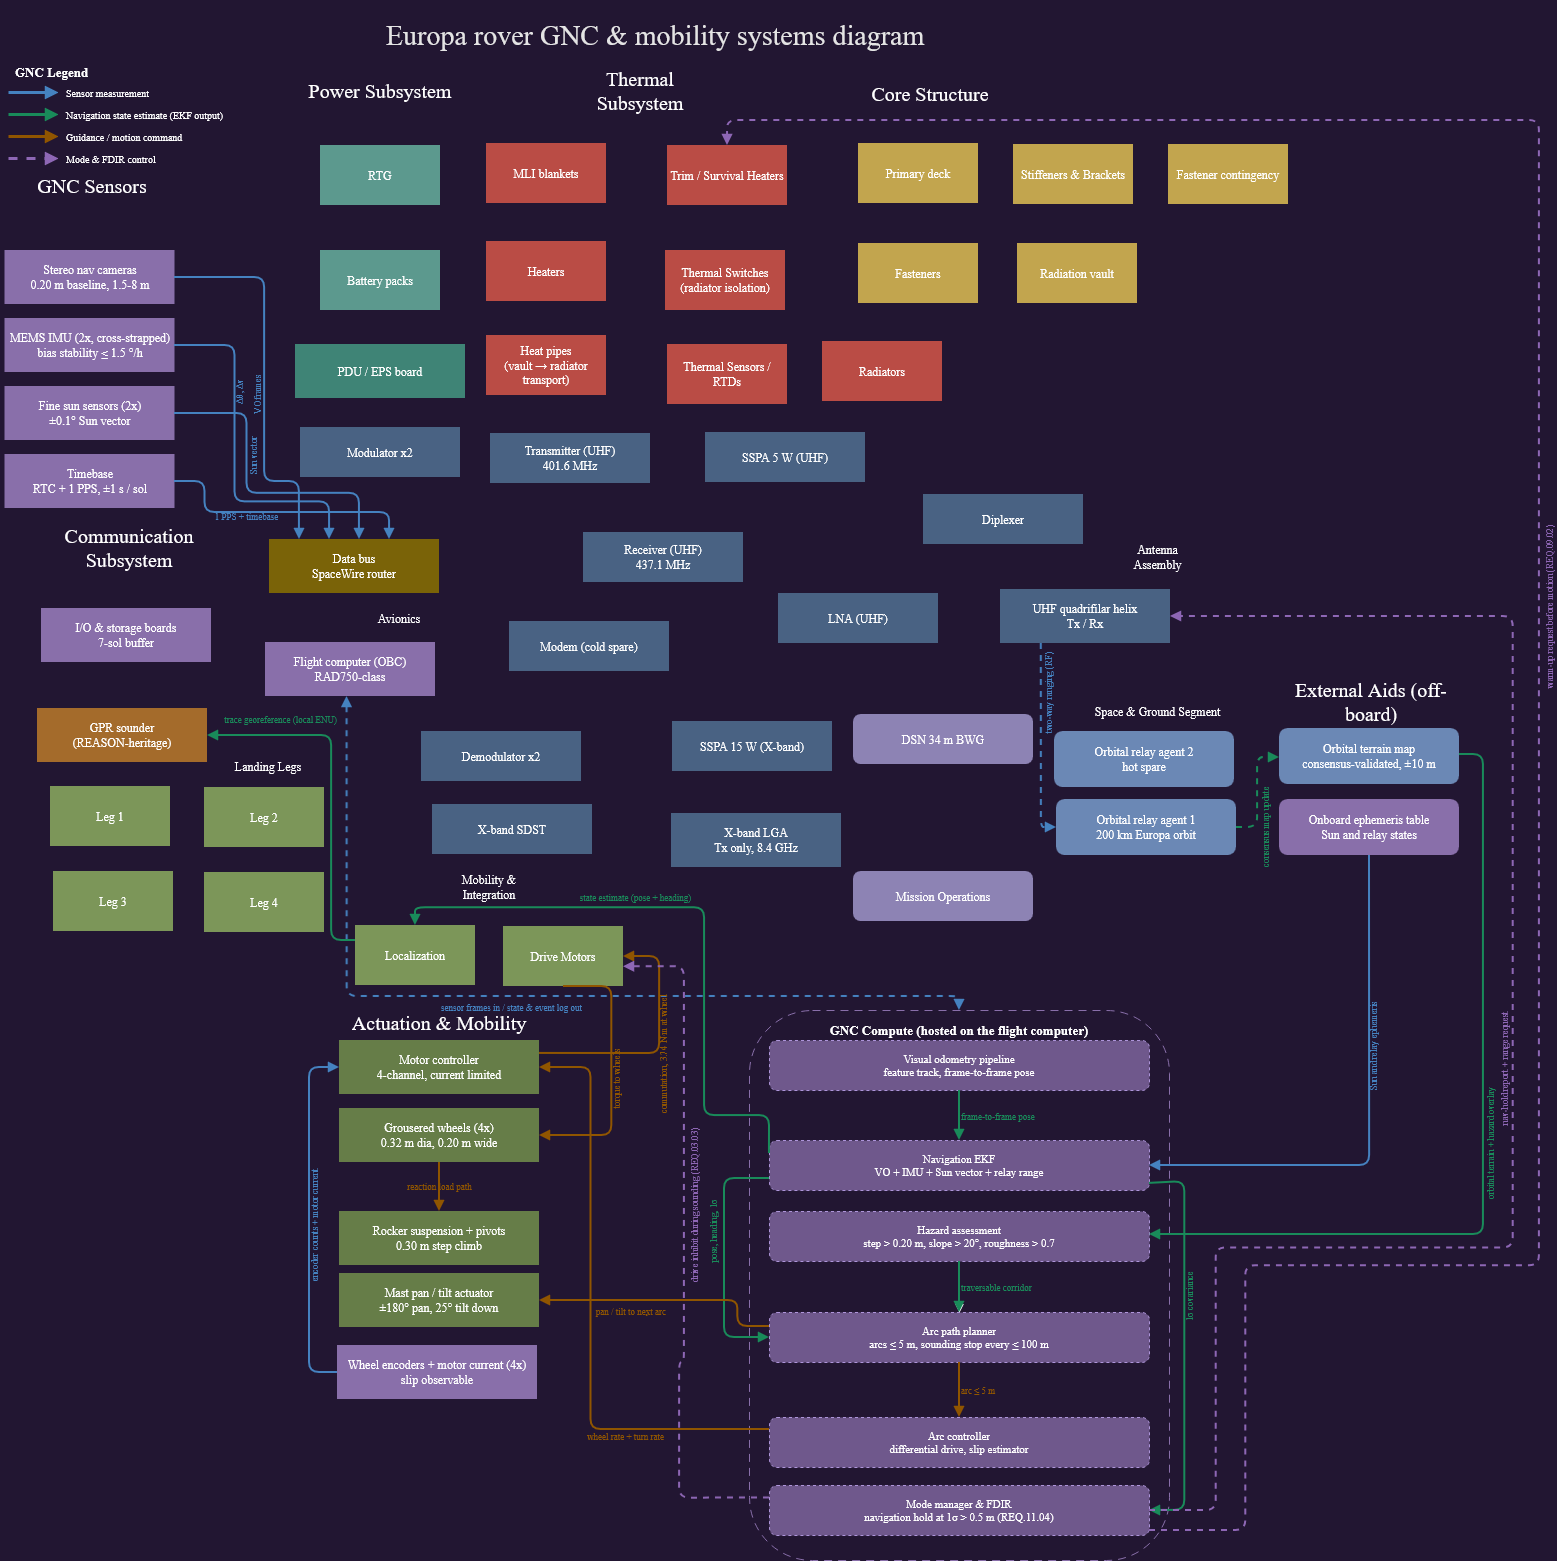
\includegraphics[width=0.95\textwidth]{figures/gnc_systems_diagram.png}
    \caption{GNC and mobility systems diagram: sensor suite, GNC compute stack (visual odometry
    $\to$ navigation EKF $\to$ hazard assessment $\to$ arc planner $\to$ arc controller $\to$
    mode manager/FDIR), and actuation/mobility hardware.}
    \label{fig:gnc-diagram}
\end{figure}

\subsection{Command and Data Handling (CDH)}

\subsubsection{CDH Requirements}
\begin{itemize}[leftmargin=*]
    \item \reqid{REQ.03.04}: Retain $\geq 7$ sols of uncompressed radar trace data onboard;
    apply lossless compression at $\geq 2{:}1$ to all Radar\_Traces records before inter-agent
    relay transmission. (CDH, Science/Payload, COMMs)
    \item \reqid{REQ.04.01}: Support mesh-network consensus on shared terrain maps within
    $\leq 10$~minutes under degraded ($\leq 30\%$ packet loss) link conditions. (CDH, COMMs)
    \item \reqid{REQ.05.02}: Detect and autonomously recover from a single-event latch-up in
    any processor core within $30$~s of occurrence, restoring nominal operations without ground
    intervention, and log each event to non-volatile memory with a timestamp and affected core
    identifier. (CDH, Electronics)
    \item \reqid{REQ.12.01}: Provide $\geq 250$~MIPS of radiation-hardened processing
    throughput with $\geq 30\%$ processor duty-cycle and volatile-memory margin at the
    worst-case concurrent GNC compute load (visual odometry, hazard assessment, navigation EKF)
    within a single $5$~m drive-arc cycle. (CDH)
    \item \reqid{REQ.12.02}: Provide $\geq 1$~GB of EDAC-protected non-volatile mass storage
    sized to $7$ sols of raw data at the $91.9$~MB/sol generation rate with $\geq 30\%$ margin,
    applying a science-priority retention policy that preserves NOMINAL-flagged radar traces and
    their paired localization records once remaining capacity falls below $10\%$. (CDH)
    \item \reqid{REQ.12.03}: Move all payload and navigation data on a cross-strapped
    SpaceWire primary bus $\geq 20$~Mbps, with an independent RS-422 command/telemetry path
    $\geq 115.2$~kbps that remains available with the primary bus failed. (CDH)
    \item \reqid{REQ.12.04}: Timestamp every record against a single onboard timebase held to
    $\pm 1$~s absolute per sol and $\pm 10$~ms record-to-record, framed with a trace identifier,
    sol index, and CCSDS-compliant packet header. (CDH)
\end{itemize}

\textbf{Resolved.} An earlier draft of the master spreadsheet had REQ.05.02's literal ``shall''
statement giving a $330$~s latch-up recovery bound while its own reasoning field, testing method,
and verification/validation plan all stated $30$~s instead. The updated master spreadsheet
(\textit{documents/Space Robotics Mission Sheet.xlsx}) now states $30$~s consistently across the
requirement statement, reasoning, and V\&V fields, matching the completed CDH design below
(Figure~\ref{fig:cdh-diagram}).

\subsubsection{CDH Architecture \& Assumptions}
The flight computer is a RAD750-class single-board computer, mounted inside the radiation vault
(Section~7.3, REQ.07.03) alongside dedicated I/O and mass-storage boards, and it hosts the entire
CDH function as well as the GNC compute stack described in Section~7.7. All payload and
navigation data move on a cross-strapped SpaceWire router bus rated $\geq 20$~Mbps: sustained
rover-wide generation is only $6.3$~kbps in idle modes, but a $1.57$~MB stereo pair read out in
about $2$~s during Traverse is a $6.3$~Mbps burst, and $20$~Mbps clears that with a factor of
$3.2$ to spare (REQ.12.03). An independent RS-422 command and telemetry path ($\geq 115.2$~kbps)
carries safe-mode telemetry directly from the flight computer to the X-band SDST, bypassing the
SpaceWire bus entirely, so a single bus failure cannot also take down the contingency beacon
(REQ.10.03) that the comms architecture depends on as a relay-loss fallback.

Every record is timestamped against a single onboard timebase (RTC plus a $1$~PPS distribution)
held to $\pm 1$~s absolute per sol and $\pm 10$~ms record-to-record, and framed with a trace
identifier, sol index, and CCSDS-compliant header (REQ.12.04): this is what lets the ground
segment reassemble the Radar\_Traces, Localization\_Log, and Terrain\_and\_Health record sets by
identifier alone after a lossy pass, rather than depending on packet arrival order. A memory
scrubber runs a full EDAC scrub of mass memory on an hourly cycle, and the mode manager/FDIR
function isolates a faulted data bus within $\leq 100$~ms and drives safe-mode entry (REQ.08.03),
detecting and recovering from a processor single-event latch-up within $30$~s of occurrence
(REQ.05.02). Figure~\ref{fig:cdh-diagram} traces the full CDH core: SpaceWire interface,
processing allocation, RS-422 backup, timebase/framing, EDAC/scrubbing, and mode manager/FDIR on
one side; mass memory, the lossless compressor, OBC staging RAM, the downlink scheduler,
science-priority retention, and the contingency-beacon fallback on the other, against every
subsystem that feeds it data or draws on its outputs.

\begin{figure}[H]
    \centering
    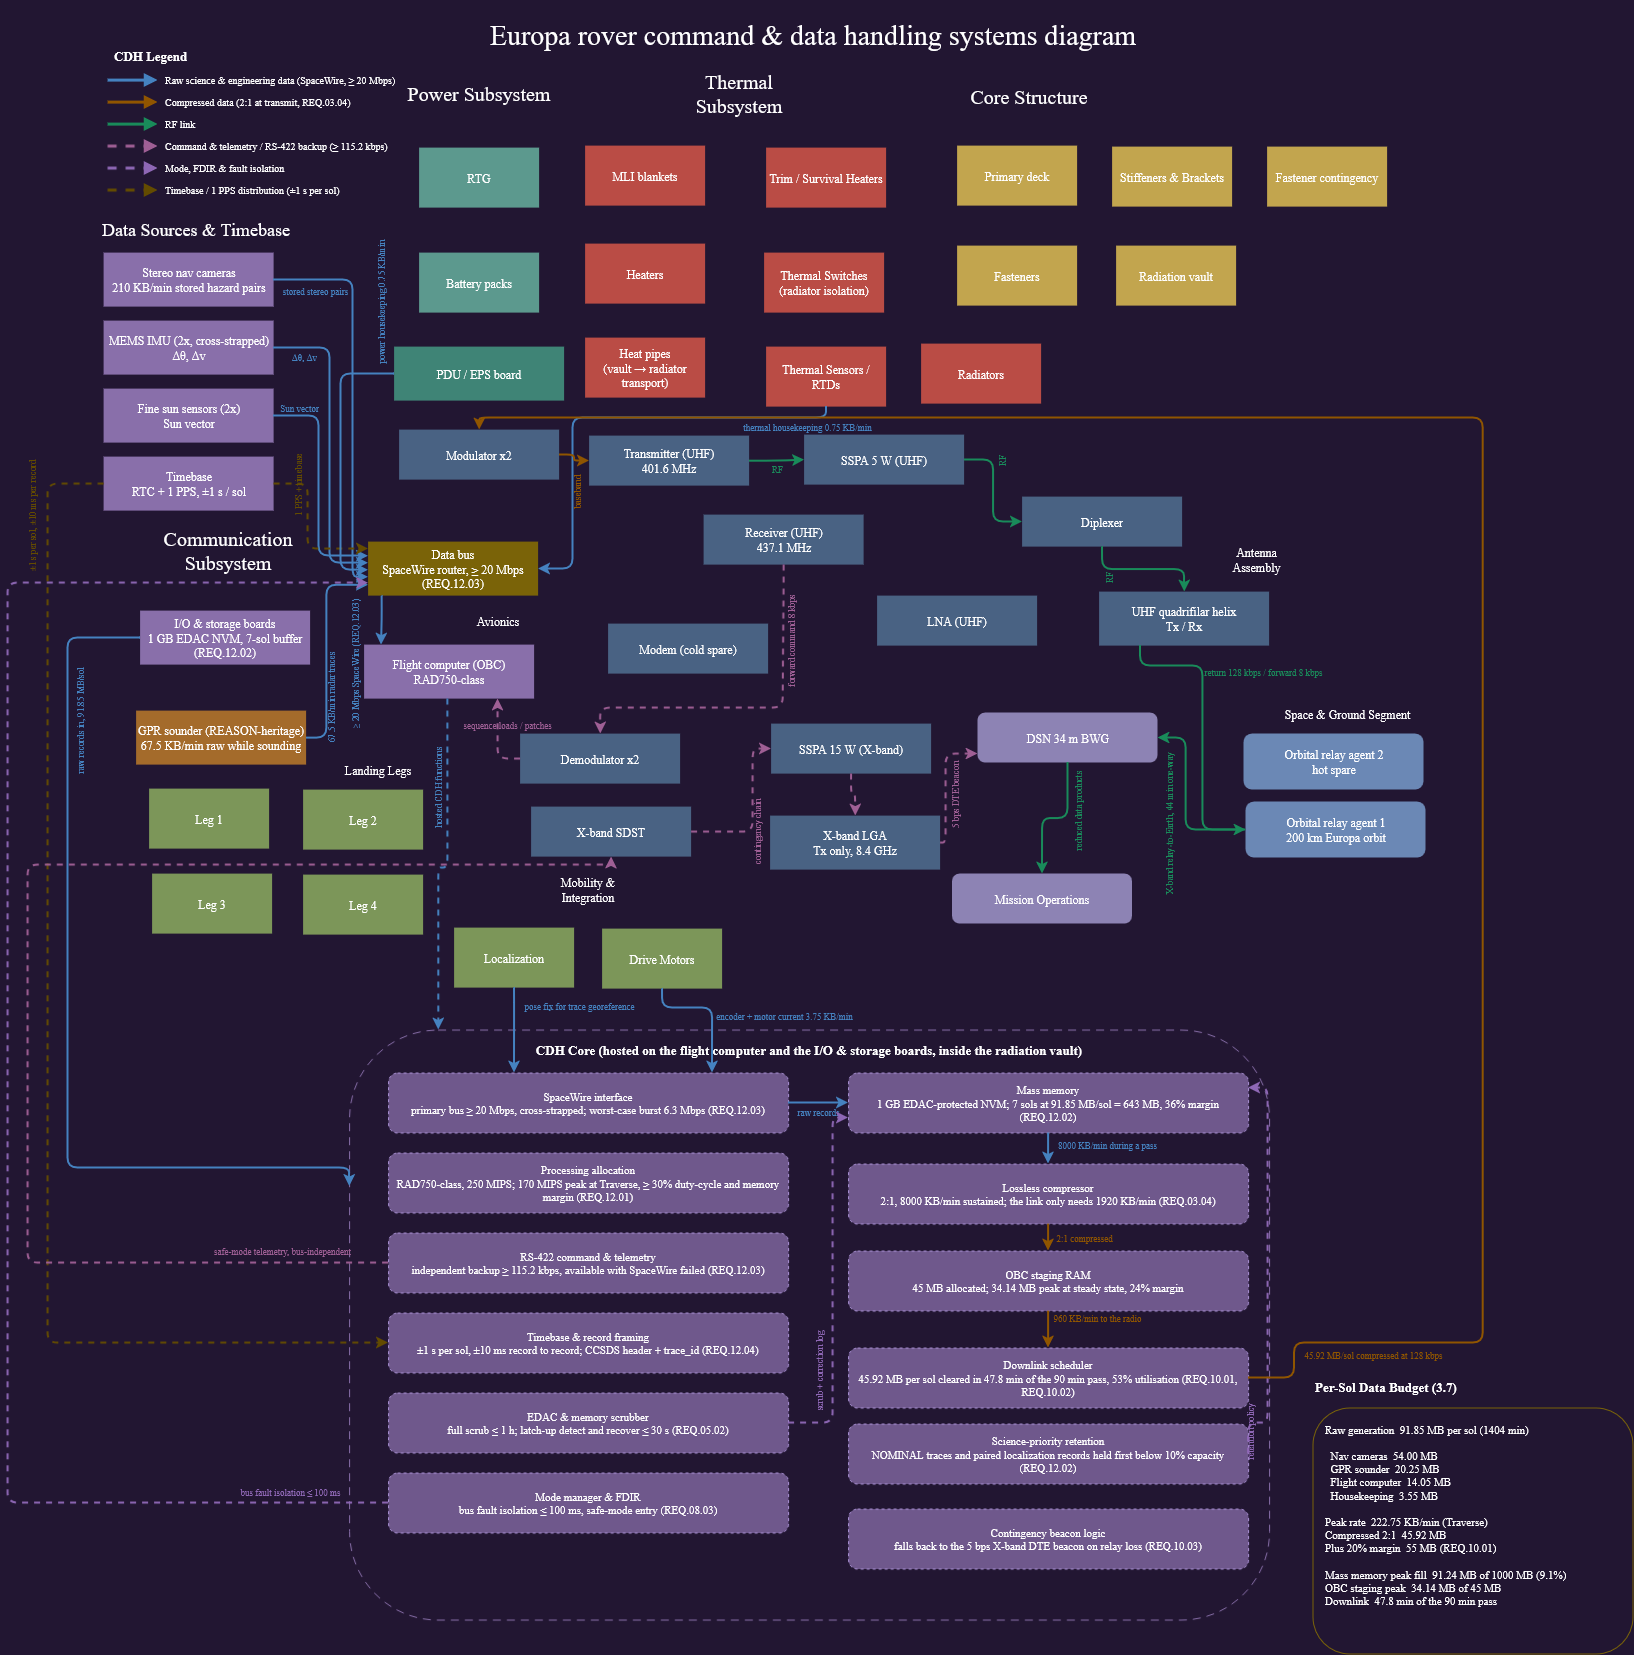
\includegraphics[width=0.95\textwidth]{figures/cdh_systems_diagram.png}
    \caption{CDH systems diagram: data sources and timebase, the SpaceWire/RS-422 avionics core
    hosted on the RAD750-class flight computer, the mass-memory/compression/downlink pipeline,
    and the per-sol data budget (Section~7.7, REQ.03.04, REQ.05.02, REQ.10.01--REQ.10.03,
    REQ.12.01--REQ.12.04).}
    \label{fig:cdh-diagram}
\end{figure}

\subsubsection{Data Budget and Storage Strategy}
Table~\ref{tab:cdh-data-budget} breaks the $91.85$~MB/sol raw-generation figure down by source.
Nav-camera stereo hazard pairs dominate the budget even though they are the most compressible and
most re-collectable product on board: the rover can re-image ground it drives again, but a
discarded NOMINAL-flagged radar trace and its paired localization record cannot be recovered
without re-driving the transect. That asymmetry is exactly why REQ.12.02's science-priority
retention policy protects radar traces and their position fixes ahead of everything else once
remaining mass-memory capacity drops below $10\%$.

\begin{table}[H]
\centering
\small
\begin{tabular}{lr}
\toprule
\textbf{Source} & \textbf{Volume (MB/sol)} \\
\midrule
Nav cameras (stereo hazard pairs) & 54.00 \\
GPR sounder (radar traces) & 20.25 \\
Flight computer (state/sequencing) & 14.05 \\
Housekeeping (thermal/power/comms telemetry) & 3.55 \\
\midrule
\textbf{Total raw generation} & \textbf{91.85} \\
\bottomrule
\end{tabular}
\caption{Per-sol raw data generation by source.}
\label{tab:cdh-data-budget}
\end{table}

Generation rate is far from uniform across modes (Table~\ref{tab:cdh-mode-rates}): Traverse is the
binding case at $222.75$~KB/min, driven by the nav-camera stereo pairs and the GNC compute
allocation running together, while Night Low-Power and Battery Emergency fall to single digits.
Radar Sounding and Traverse Planning tie at $76.5$~KB/min because the sounder never runs
concurrently with drive motors (REQ.03.03's stop-and-sound logic), so its $67.5$~KB/min raw trace
rate is the whole story in that mode, mirrored by the flight computer's own $30$~KB/min
map-generation-and-consensus compute load carried into Traverse Planning at $15$~KB/min plus
imagery.

\begin{table}[H]
\centering
\small
\begin{tabular}{lr}
\toprule
\textbf{Operational Mode} & \textbf{Avg. Data Generation (KB/min)} \\
\midrule
Traverse & 222.75 \\
Radar Sounding & 76.5 \\
Traverse Planning & 76.5 \\
Map Gen \& Consensus & 33.0 \\
Systems Warm-Up & 9.0 \\
Comms Relay Pass & 6.75 \\
Thermal Emergency & 5.25 \\
Night Low-Power & 3.0 \\
Battery Emergency & 2.25 \\
\bottomrule
\end{tabular}
\caption{Average data-generation rate by operational mode.}
\label{tab:cdh-mode-rates}
\end{table}

Sized against a $1$~GB EDAC-protected NAND storage board, $7$ sols of raw data is $643$~MB
(REQ.03.04's storage horizon), which is $64\%$ of device capacity and leaves $36\%$ margin:
the figure REQ.12.02 uses as its storage-sizing floor. In nominal operation, though, the buffer
never gets close to that: the downlink scheduler clears each sol's compressed volume during the
following relay pass, so mass memory peaks at only about $91.2$~MB ($9.1\%$ of capacity) before
the next contact drains it, and the full $643$~MB horizon exists purely as an outage reserve if
one or more relay passes are missed. The lossless compressor runs at $2{:}1$ (REQ.03.04) with
$8{,}000$~KB/min of throughput margin against a sustained need of only about $1{,}920$~KB/min,
producing $45.92$~MB of compressed data per sol; adding REQ.10.01's $20\%$ margin gives the
$\geq 55$~MB/day delivered-volume floor that sizes the $128$~kbps return link in Section~7.6.
Compressed data queues in $45$~MB of OBC staging RAM, which peaks at $34.14$~MB ($24\%$ margin)
at steady state: the tightest margin anywhere in the CDH design and the first place to look if
the return link ever slows down or a relay outage lets a backlog build. The downlink scheduler
clears the full $45.92$~MB in $47.8$ of the $90$-minute relay pass ($53\%$ utilization,
REQ.10.01/REQ.10.02), and if both relay links are lost the contingency-beacon logic falls back to
the $5$~bps X-band direct-to-Earth beacon from Section~7.6 (REQ.10.03) rather than waiting on the
primary science-data path.

\subsubsection{CDH Trade Study}
\textbf{Study:} Analysis of the onboard flight computer and mass-storage architecture.
Options were scored against five pairwise-weighted criteria (Mass $0.10$, Power Demand $0.15$,
Processing Throughput $0.20$, Radiation Durability $0.30$, Reliability/TRL $0.25$).

\begin{table}[H]
\centering
\small
\resizebox{\textwidth}{!}{%
\begin{tabular}{lccc}
\toprule
\textbf{Criterion (weight)} & \textbf{RAD750-class SBC + 1~GB rad-hard NAND} &
\textbf{RAD5545 quad-core PowerPC + 4~GB} & \textbf{COTS ARM SoC (Zynq-class) + TMR voting} \\
\midrule
Mass (0.10) & 0.40 & 0.30 & 0.50 \\
Power Demand (0.15) & 0.60 & 0.45 & 0.75 \\
Processing Throughput (0.20) & 0.60 & 1.00 & 1.00 \\
Radiation Durability (0.30) & 1.50 & 1.20 & 0.60 \\
Reliability/TRL (0.25) & 1.25 & 0.75 & 0.50 \\
\midrule
\textbf{Total Score} & \textbf{4.35} & 3.70 & 3.35 \\
\bottomrule
\end{tabular}
}
\caption{Onboard flight computer and mass-storage architecture trade study.}
\label{tab:cdh-trade}
\end{table}

\textbf{Winning option: RAD750-class SBC with a $1$~GB rad-hard NAND storage board.}
Radiation durability and flight heritage carry $55\%$ of the weight between them, and that is
what decides this. RAD750 parts are latch-up immune by process and qualified past $100$~krad
(the figure REQ.01.02 already fixes), and the part flew to Jupiter on Juno and is flying there
again on Europa Clipper; nothing else in the trade has seen this environment. Throughput is
where it gives ground: roughly $266$~MIPS at $200$~MHz against a peak load near $170$~MIPS during
Traverse, when visual odometry, hazard assessment, and the navigation EKF all run inside one arc
cycle. That leaves $36\%$ margin against the $30\%$ floor in REQ.12.01, so the answer is adequate
rather than comfortable, and it is the first term to watch if the visual-odometry pipeline grows.
The RAD5545 buys throughput the mission does not need: peak generation across the whole rover is
only $29.7$~kbps and the buffer never climbs past $9\%$ of capacity on a nominal sol, so there is
no processing or storage problem worth its extra mass and lower TRL. The COTS ARM SoC is the
tempting option and the wrong one; it wins mass, power, and throughput outright, then loses on
the one axis that ends missions here: at $20$--$50$~krad it is consumed inside the $30$-sol
surface phase even behind the vault, and TMR voting protects a running computation against
upsets while doing nothing about total dose. With a $44$-minute one-way light delay there is no
ground recovery for a part that has simply worn out.

% ====================================================
% 8. REFERENCES
% ====================================================
\newpage
\section{References}

\begin{thebibliography}{99}

\bibitem{owlDecadal}
National Academies of Sciences, Engineering, and Medicine,
\textit{Origins, Worlds, and Life: A Decadal Strategy for Planetary Science and Astrobiology
2023--2032}, The National Academies Press, Washington, D.C., 2022.
Available: \url{https://www.nationalacademies.org/read/26522}.

\bibitem{stmdShortfall}
NASA Space Technology Mission Directorate,
``Civil Space Technology Shortfall Rankings,'' NASA, Washington, D.C., Jul.\ 2024.
Available: \url{https://www.nasa.gov/wp-content/uploads/2024/07/civil-space-shortfall-ranking-july-2024.pdf}.

\bibitem{nasaSBIR}
NASA, ``FY 2026--2027 SBIR/STTR Program Solicitation, Appendix 26B-I: SBIR Topics,'' NASA Small
Business Innovation Research Program, 2025. Topic COMNAV.1.S26B.

\bibitem{jplEuropaClipper}
NASA Jet Propulsion Laboratory, ``Europa Clipper,'' JPL, Pasadena, CA.
Available: \url{https://www.jpl.nasa.gov/missions/europa-clipper/}.

\bibitem{wikiEuropaClipper}
Wikipedia contributors, ``Europa Clipper,'' \textit{Wikipedia, The Free Encyclopedia}.
Available: \url{https://en.wikipedia.org/wiki/Europa_Clipper}.

\bibitem{utigReason}
University of Texas at Austin Jackson School of Geosciences, ``Scientific Instrument Developed
by UTIG Scientists Headed to Europa,'' UT Austin, Austin, TX, Apr.\ 2025.

\bibitem{reason}
NASA, ``Radar for Europa Assessment and Sounding: Ocean to Near-surface (REASON),'' Europa
Clipper Mission. Available: \url{https://europa.nasa.gov/spacecraft/instruments/reason/}.

\bibitem{dsnHandbook}
Jet Propulsion Laboratory, ``DSN Telecommunications Link Design Handbook,'' 810-005, Rev.~E,
NASA/JPL, Pasadena, CA. Available: \url{https://deepspace.jpl.nasa.gov/dsndocs/810-005/}.

\bibitem{ccsds2111}
Consultative Committee for Space Data Systems, ``Proximity-1 Space Link Protocol: Physical
Layer,'' CCSDS 211.1-B-4, 2013.

\bibitem{ccsds1310}
Consultative Committee for Space Data Systems, ``TM Synchronization and Channel Coding,'' CCSDS
131.0-B-4, 2017.

\bibitem{electra}
C.~D.~Edwards \textit{et al.}, ``The Electra Proximity Link Payload for Mars Relay
Telecommunications and Navigation,'' Jet Propulsion Laboratory, Pasadena, CA.

\bibitem{dsnOverview}
NASA, ``Deep Space Network,'' NASA Space Communications and Navigation.
Available: \url{https://www.nasa.gov/communicating-with-missions/dsn/}.

\bibitem{kietzig}
A.-M.\ Kietzig, S.~G.\ Hatzikiriakos, and P.~Englezos, ``Physics of Ice Friction,'' \textit{Journal
of Applied Physics}, vol.\ 107, no.\ 8, 081101, 2010.

\bibitem{maimone}
M.~Maimone, Y.~Cheng, and L.~Matthies, ``Two Years of Visual Odometry on the Mars Exploration
Rovers,'' \textit{Journal of Field Robotics}, vol.\ 24, no.\ 3, pp.\ 169--186, 2007.

\bibitem{mslWheels}
NASA Jet Propulsion Laboratory, ``Mars Science Laboratory: Mobility System,'' JPL, Pasadena, CA.
Available: \url{https://mars.nasa.gov/msl/spacecraft/rover/wheels/}.

\bibitem{roverComponents}
NASA Science, ``Perseverance Rover Components,'' NASA Science Mission Directorate, Jul.\ 22,
2025. Available: \url{https://science.nasa.gov/mission/mars-2020-perseverance/rover-components/}.

\end{thebibliography}

% ====================================================
% APPENDICES
% ====================================================
\newpage
\begin{appendices}

\section{Extended Trade Study Tables}
The Structures (Table~\ref{tab:structures-trade}), Power (Table~\ref{tab:power-trade}), Thermal
(Table~\ref{tab:thermal-trade}), Communications (Table~\ref{tab:comms-trade}), GNC
(Table~\ref{tab:gnc-trade}), and CDH (Table~\ref{tab:cdh-trade}) trade studies in Section~7
already reproduce the full pairwise-weighted decision matrices used in the source spreadsheets.
Each uses the same methodology: criteria weighted by pairwise comparison in $0.25$ increments
(summing to $1$ per pair, normalized to sum to unity across all criteria), and options scored
$1$--$5$ against a per-criterion rubric before weighting. Only the Structures and CDH scoring
rubrics' full $1$--$5$ band definitions are omitted here for length; they are reproduced in the
source Decision Matrix / Trade Study PDFs in each subsystem's folder.

\section{Full Requirements Spreadsheet}
Table~\ref{tab:master-reqs} consolidates every requirement identified across the source
assignments (REQ.01.01 through REQ.12.04), with owning subsystem(s). Full justification,
verification, and validation text for each requirement is maintained in the master spreadsheet
(\textit{documents/Space Robotics Mission Sheet.xlsx}, the cumulative requirements sheet, carried
in this report's own folder) and is not fully duplicated here for length; representative
full-text entries appear in Sections~3.3 and 7.

\begin{longtable}{p{1.6cm}p{8.6cm}p{3cm}}
\toprule
\textbf{ID} & \textbf{Statement (condensed)} & \textbf{Subsystem(s)} \\
\midrule
\endhead
REQ.01.01 & Full autonomy for entire surface mission; no real-time Earth uplink. & System \\
REQ.01.02 & Survive $\geq 100$~krad TID over mission lifetime. & System, Electronics, Power \\
REQ.01.03 & $\geq 2$ active relay nodes at all times during surface ops. & System, COMMs \\
REQ.02.01 & Localization $\pm 0.5$~m over any $50$~m segment, no GPS. & Mobility, GNC \\
REQ.03.01 & GPR resolves ice thickness $\pm 10\%$, 1--30~km depth, $\geq 100$~m resolution. &
Science/Payload, Power \\
REQ.03.02 & Antenna boresight $\pm 5^\circ$ nadir; halt above $20^\circ$ slope. &
Science/Payload, Structures, Mobility \\
REQ.03.03 & Peak power reserved for radar pulses; drive shutdown during sounding. &
Science/Payload, Power, Mobility \\
REQ.03.04 & $\geq 7$-sol onboard storage; $\geq 2{:}1$ lossless compression before relay. &
Science/Payload, COMMs, CDH \\
REQ.04.01 & Mesh consensus $\leq 10$~min under $\leq 30\%$ packet loss. & COMMs, CDH \\
REQ.05.01 & Avionics/battery $0$--$40^\circ$C active, $>-20^\circ$C night mode. & Thermal,
Power, Structures \\
REQ.05.02 & Detect/recover from a processor latch-up autonomously within $30$~s, log event w/
timestamp \& core ID. & CDH, Electronics \\
REQ.05.03 & Per-sol draw $\leq 90\%$ RTG output; $\geq 10\%$ margin reserve. & Power, CDH,
Thermal, Mobility \\
REQ.06.01 & $\geq 100$~m/sol autonomous traverse; sounding stop $\leq 100$~m intervals. &
Mobility \\
REQ.06.02 & Onboard site-selection algorithm autonomously evaluates each NOMINAL-flagged radar
trace against the cryobot insertion criteria (ice $<5$~km, slope $<20^\circ$, roughness $<0.7$)
and flags a candidate site within one sol of the criteria first being satisfied, without ground
intervention. & Science/Payload, Mobility, GNC \\
REQ.06.03 & Daily summary packet autonomously sent within 2~hr of sol's radar window. & COMMs,
CDH, Science/Payload \\
REQ.07.01 & Landing legs accommodate $12g$ vertical / $6g$ lateral touchdown loads across four
footpads, no permanent deformation. & Structures, Mobility, GNC \\
REQ.07.02 & Structural materials remain in-spec at $90$~K over 30-sol lifetime. & Structures,
Thermal, Power \\
REQ.07.03 & Radiation vault attenuates dose to $\leq 1$~krad/sol at electronics level within
structures mass allocation. & Structures, Power, Electronics, CDH \\
REQ.08.01 & MMRTG $\geq 110$~We BOL, $\geq 80$~We continuous, $\geq 1.9$~kWh/sol. & Power,
Thermal, System \\
REQ.08.02 & Battery $\geq 2.4$~kWh usable; $\geq 12$~hr night survival; $>-20^\circ$C. & Power,
Thermal \\
REQ.08.03 & PDU isolates a faulted load bus within $100$~ms; critical loads uninterrupted; fault
logged autonomously. & Power, CDH, Electronics \\
REQ.09.01 & Reject $\leq 500$~W; vault $<40^\circ$C during peak ops. & Thermal, Electronics,
Power, CDH \\
REQ.09.02 & Preheat actuators $>-40^\circ$C within $60$~min of cold start. & Thermal, Mobility,
Structures \\
REQ.09.03 & MLI + RTG waste heat bound survival heaters $\leq 50$~W. & Thermal, Power,
Structures \\
REQ.10.01 & $\geq 55$~MB/day compressed; $\geq 128$~kbps return / $\geq 8$~kbps forward. &
COMMs, CDH, Science/Payload, Power \\
REQ.10.02 & $\geq 2$ relay contacts/sol, $\geq 90$~min total; latency $\leq 26$~hr. & COMMs,
CDH, Science/Payload, GNC \\
REQ.10.03 & Link $\geq 3$~dB margin @ $588$~km worst case; X-band DTE beacon $\geq 5$~bps
fallback. & COMMs, Power, Structures, CDH \\
REQ.11.01 & Attitude $\pm 0.5^\circ$ roll/pitch, heading $\pm 0.25^\circ$ per arc, sun-sensor
fix every $\leq 5$~m. & GNC, Mobility, Science/Payload, CDH \\
REQ.11.02 & Hazard assessment $\geq 8$~m lookahead; reject step $>0.20$~m / slope $>20^\circ$ /
roughness $>0.7$. & GNC, Mobility, Science/Payload, CDH \\
REQ.11.03 & Cross-track $\leq 0.5$~m/50~m; waypoint $\pm 0.5$~m; differential drive + slip
estimate. & GNC, Mobility, Science/Payload \\
REQ.11.04 & Navigation hold if $1\sigma > 0.5$~m; re-init via 2-relay ranging + map
correlation. & GNC, COMMs, CDH, Mobility \\
REQ.12.01 & $\geq 250$~MIPS rad-hard throughput; $\geq 30\%$ duty-cycle/memory margin at
peak GNC compute load per arc. & CDH \\
REQ.12.02 & $\geq 1$~GB EDAC NVM sized to 7 sols @ $91.9$~MB/sol, $\geq 30\%$ margin;
science-priority retention below $10\%$ capacity. & CDH \\
REQ.12.03 & SpaceWire primary bus $\geq 20$~Mbps, cross-strapped; independent RS-422
backup $\geq 115.2$~kbps survives primary-bus failure. & CDH \\
REQ.12.04 & Timebase $\pm 1$~s/sol, $\pm 10$~ms record-to-record; CCSDS header + trace ID
framing. & CDH \\
\bottomrule
\caption{Condensed master requirements list, REQ.01.01--REQ.12.04.}
\label{tab:master-reqs}
\end{longtable}

REQ.06.02, REQ.07.01, REQ.07.03, and REQ.08.03 have all been checked directly against the
authoritative \textit{documents/Space Robotics Mission Sheet.xlsx}: REQ.06.02's condensed entry
above now carries the literal statement text (it was previously a reconstruction that also
dropped the one-sol response-time clause); REQ.07.01 and REQ.08.03 were already worded
consistently with the master sheet and needed no change; and REQ.07.03's vault mass allocation
now reads $25.75$~kg, matching the Structure subsystem total in the mass budget (see Section~7.3).

\section{Sample Datasets}
A 20-trace Radar\_Traces export (Sol 1, \texttt{TR-0001}--\texttt{TR-0020}) and the complete
Daily\_Summary export (Sol 1--2, the full extent of that sheet's current contents), both pulled
directly from \textit{Data Product Space Robotics.xlsx}, are reproduced in
Section~6.2 (Tables~\ref{tab:sample-record}, \ref{tab:sample-record-2},
and~\ref{tab:sample-daily}) rather than duplicated here for length.

\section{Tools Used}
This report was assembled with the assistance of Claude (Anthropic), which synthesized and
reorganized the author's prior assignment deliverables into the Section 4.1 template. Per-assignment
AI-use disclosures carried over from the source documents are consolidated below.

\begin{itemize}[leftmargin=*]
    \item \textbf{2.1 Designing a Data Product:} ``Artificial intelligence tools were used to
    verify that the technical statements, parameter values, and requirement references made in
    this document are consistent with the background research on Europa ice-shell radar
    sounding, cryobot mission concepts, and planetary robotics requirements engineering. AI also
    generated fake data to demonstrate the data being recorded.''
    \item \textbf{2.3 ConOps Sketch:} ``AI was used to check grammar and rephrase for better
    wording. The prompt used was: `Please check grammar, cohesiveness and correct wording of
    the following.'''
    \item \textbf{3.4 Point-Mass Thermal Equilibrium:} ``AI was used to fact-check the results.''
    \item \textbf{3.5 Link Budget:} ``I used AI to check the arithmetic behind each link budget
    term and to cross-check the assumed parameters against published Electra and DSN performance
    data. I picked the architecture and the parameters myself, and I set the margin the same
    way.''
    \item \textbf{3.6 Mobility Solution:} ``I used AI to check the arithmetic behind the
    traction, torque, and localization error budget numbers, and to cross-check the
    low-temperature ice friction values against published measurements. The mobility
    architecture is all mine. Diagram generated using Claude Opus 5.''
    \item \textbf{1.3 Deep Dive into a Robotic Mission:} ``Claude Opus 5 (Anthropic) was used
    to compare this paper against the assignment rubric and provide a grade estimate.''
\end{itemize}

\textbf{3.2 Structures and Mechanisms Design (dedicated AI Use Disclosure):}
``The attached rover sketch was generated as an SVG graphic using Claude (model: Claude Opus 5),
an AI assistant developed by Anthropic, accessed through the claude.ai interface. What the AI
did: Produced the SVG drawing (linework, layout, labels, and leader lines) based on my direction.
What the AI did not do: The design content, comprising component selection, structural
configuration, materials (Al 7075-T73 struts, Ti-6Al-4V vault), payload (REASON-heritage GPR),
and requirements traceability, comes from my own prior coursework (requirements, trade study, and mass budget
for this mission). The AI drew from those documents rather than originating the design. Process:
The sketch went through several revision cycles that I directed, including corrections to the
suspension architecture, GPR mounting orientation (nadir-pointing, belly-mounted), sensor mast
structure, RTG mounting, and the landing strut separation mechanism. I reviewed the final output
for accuracy against my mission design.''

\end{appendices}

\end{document}
